%%%%%%%%%%%%%%%%%%%%%%%%%%%%%%%%%%%%%%%%%
% Masters/Doctoral Thesis 
% LaTeX Template
% Version 2.2 (21/11/15)
%
% This template has been downloaded from:
% http://www.LaTeXTemplates.com
%
% Version 2.x major modifications by:
% Vel (vel@latextemplates.com)
%
% This template is based on a template by:
% Steve Gunn (http://users.ecs.soton.ac.uk/srg/softwaretools/document/templates/)
% Sunil Patel (http://www.sunilpatel.co.uk/thesis-template/)
%
% Template license:
% CC BY-NC-SA 3.0 (http://creativecommons.org/licenses/by-nc-sa/3.0/)
%
%%%%%%%%%%%%%%%%%%%%%%%%%%%%%%%%%%%%%%%%%

%----------------------------------------------------------------------------------------
%	PACKAGES AND OTHER DOCUMENT CONFIGURATIONS
%----------------------------------------------------------------------------------------

\documentclass[
11pt, % The default document font size, options: 10pt, 11pt, 12pt
%oneside, % Two side (alternating margins) for binding by default, uncomment to switch to one side
english, % ngerman for German
singlespacing, % Single line spacing, alternatives: onehalfspacing or doublespacing
%draft, % Uncomment to enable draft mode (no pictures, no links, overfull hboxes indicated)
%nolistspacing, % If the document is onehalfspacing or doublespacing, uncomment this to set spacing in lists to single
%liststotoc, % Uncomment to add the list of figures/tables/etc to the table of contents
%toctotoc, % Uncomment to add the main table of contents to the table of contents
parskip, % Uncomment to add space between paragraphs
%nohyperref, % Uncomment to not load the hyperref package
headsepline, % Uncomment to get a line under the header
]{MastersDoctoralThesis} % The class file specifying the document structure

\usepackage[utf8]{inputenc} % Required for inputting international characters
\usepackage[T1]{fontenc} % Output font encoding for international characters

\usepackage{palatino} % Use the Palatino font by default

\usepackage[backend=bibtex,style=authoryear,natbib=true]{biblatex} % User the bibtex backend with the authoryear citation style (which resembles APA)

\addbibresource{example.bib} % The filename of the bibliography

\usepackage[autostyle=true]{csquotes} % Required to generate language-dependent quotes in the bibliography

%----------------------------------------------------------------------------------------
%	MARGIN SETTINGS
%----------------------------------------------------------------------------------------

\geometry{
	paper=a4paper, % Change to letterpaper for US letter
	inner=2.5cm, % Inner margin
	outer=3.8cm, % Outer margin
	bindingoffset=2cm, % Binding offset
	top=1.5cm, % Top margin
	bottom=1.5cm, % Bottom margin
	%showframe,% show how the type block is set on the page
}

%----------------------------------------------------------------------------------------
%	THESIS INFORMATION
%----------------------------------------------------------------------------------------

\thesistitle{A scalable distributed autonomy system for fractionated satellite missions} % Your thesis title, this is used in the title and abstract, print it elsewhere with \ttitle
\supervisor{Dr. Eduard \textsc{Alarc\'on Cot}} % Your supervisor's name, this is used in the title page, print it elsewhere with \supname
\examiner{} % Your examiner's name, this is not currently used anywhere in the template, print it elsewhere with \examname
\degree{Degree in Science and Telecommunication Technologies Engineering} % Your degree name, this is used in the title page and abstract, print it elsewhere with \degreename
\author{Santiago \textsc{Rodrigo Mu\~noz}} % Your name, this is used in the title page and abstract, print it elsewhere with \authorname
\addresses{} % Your address, this is not currently used anywhere in the template, print it elsewhere with \addressname

\subject{} % Your subject area, this is not currently used anywhere in the template, print it elsewhere with \subjectname
\keywords{} % Keywords for your thesis, this is not currently used anywhere in the template, print it elsewhere with \keywordnames
\university{\href{http://www.upc.edu}{Universitat Polit\`ecnica de Catalunya}} % Your university's name and URL, this is used in the title page and abstract, print it elsewhere with \univname
\department{\href{http://www.etsetb.upc.edu}{Escola T\`ecnica d'Enginyeria de Telecomunicaci\'o de Barcelona}} % Your department's name and URL, this is used in the title page and abstract, print it elsewhere with \deptname
\group{\href{http://www.etsetb.upc.edu}{Escola T\`ecnica d'Enginyeria de Telecomunicaci\'o de Barcelona}} % Your research group's name and URL, this is used in the title page, print it elsewhere with \groupname
\faculty{\href{http://www.etsetb.upc.edu}{Escola T\`ecnica d'Enginyeria de Telecomunicaci\'o de Barcelona}} % Your faculty's name and URL, this is used in the title page and abstract, print it elsewhere with \facname

\hypersetup{pdftitle=\ttitle} % Set the PDF's title to your title
\hypersetup{pdfauthor=\authorname} % Set the PDF's author to your name
\hypersetup{pdfkeywords=\keywordnames} % Set the PDF's keywords to your keywords

\begin{document}

\frontmatter % Use roman page numbering style (i, ii, iii, iv...) for the pre-content pages

\pagestyle{plain} % Default to the plain heading style until the thesis style is called for the body content

%----------------------------------------------------------------------------------------
%	TITLE PAGE
%----------------------------------------------------------------------------------------

\begin{titlepage}
\begin{center}

\textsc{\LARGE \univname}\\[1.5cm] % University name

\HRule \\[0.4cm] % Horizontal line
{\huge \bfseries \ttitle}\\[0.2cm] % Thesis title
\HRule \\[3.5cm] % Horizontal line
 
\large \textit{A Degree Thesis Submitted to the Faculty of the \facname ~by}\\[0.2cm]

\Large \textbf{\authorname}\\[0.2cm]

\large \textit{in partial fulfilment of the requirements\\ for the}\\[0.5cm]

\Large \textbf{\degreename}\\[2.0cm] % University requirement text

\emph{Advisors:} \\
\large \textbf{Carles \textsc{Araguz L\'opez}}\\\textbf{Dr. Elisenda \textsc{Bou Balust}}\\[1.0cm]

\Large \emph{Reporting advisor (ponent):} \\
\large \textbf{\supname}\\[1.0cm]
 
{\large \today}\\[2cm] % Date
%\includegraphics{Logo} % University/department logo - uncomment to place it
 
\vfill
\end{center}
\end{titlepage}

%%----------------------------------------------------------------------------------------
%%	DECLARATION PAGE
%%----------------------------------------------------------------------------------------
%
%\begin{declaration}
%\addchaptertocentry{\authorshipname}
%
%\noindent I, \authorname, declare that this thesis titled, \enquote{\ttitle} and the work presented in it are my own. I confirm that:
%
%\begin{itemize} 
%\item This work was done wholly or mainly while in candidature for a research degree at this University.
%\item Where any part of this thesis has previously been submitted for a degree or any other qualification at this University or any other institution, this has been clearly stated.
%\item Where I have consulted the published work of others, this is always clearly attributed.
%\item Where I have quoted from the work of others, the source is always given. With the exception of such quotations, this thesis is entirely my own work.
%\item I have acknowledged all main sources of help.
%\item Where the thesis is based on work done by myself jointly with others, I have made clear exactly what was done by others and what I have contributed myself.\\
%\end{itemize}
% 
%\noindent Signed:\\
%\rule[0.5em]{25em}{0.5pt} % This prints a line for the signature
% 
%\noindent Date:\\
%\rule[0.5em]{25em}{0.5pt} % This prints a line to write the date
%\end{declaration}
%
%\cleardoublepage

%----------------------------------------------------------------------------------------
%	DEDICATION
%----------------------------------------------------------------------------------------

\dedicatory{For/Dedicated to/To my\ldots} 

%----------------------------------------------------------------------------------------
%	ACKNOWLEDGEMENTS
%----------------------------------------------------------------------------------------

\begin{acknowledgements}
\addchaptertocentry{\acknowledgementname} % Add the acknowledgements to the table of contents

The acknowledgments and the people to thank go here, don't forget to include your project advisor\ldots

\end{acknowledgements}

%----------------------------------------------------------------------------------------
%	ABSTRACT PAGE
%----------------------------------------------------------------------------------------

\begin{abstract}
\addchaptertocentry{\abstractname} % Add the abstract to the table of contents

The Thesis Abstract is written here (and usually kept to just this page). The page is kept centered vertically so can expand into the blank space above the title too\ldots

\end{abstract}

%%%%%%%%%%%%%%%%%%%%%%%%%%%%%%%%
% INCLUIR CASTELLANO Y CATALAN %
%%%%%%%%%%%%%%%%%%%%%%%%%%%%%%%%

%----------------------------------------------------------------------------------------
%	LIST OF CONTENTS/FIGURES/TABLES PAGES
%----------------------------------------------------------------------------------------

\tableofcontents % Prints the main table of contents

\listoffigures % Prints the list of figures

\listoftables % Prints the list of tables

%%----------------------------------------------------------------------------------------
%%	ABBREVIATIONS
%%----------------------------------------------------------------------------------------
%
%\begin{abbreviations}{ll} % Include a list of abbreviations (a table of two columns)
%
%\textbf{LAH} & \textbf{L}ist \textbf{A}bbreviations \textbf{H}ere\\
%\textbf{WSF} & \textbf{W}hat (it) \textbf{S}tands \textbf{F}or\\
%
%\end{abbreviations}
%
%%----------------------------------------------------------------------------------------
%%	PHYSICAL CONSTANTS/OTHER DEFINITIONS
%%----------------------------------------------------------------------------------------
%
%\begin{constants}{lr@{${}={}$}l} % The list of physical constants is a three column table
%
%% The \SI{}{} command is provided by the siunitx package, see its documentation for instructions on how to use it
%
%	Speed of Light & $c_{0}$ & \SI{2.99792458e8}{\meter\per\second} (exact)\\
%%Constant Name & $Symbol$ & $Constant Value$ with units\\
%
%\end{constants}
%
%%----------------------------------------------------------------------------------------
%%	SYMBOLS
%%----------------------------------------------------------------------------------------
%
%\begin{symbols}{lll} % Include a list of Symbols (a three column table)
%
%$a$ & distance & \si{\meter} \\
%$P$ & power & \si{\watt} (\si{\joule\per\second}) \\
%%Symbol & Name & Unit \\
%
%\addlinespace % Gap to separate the Roman symbols from the Greek
%
%$\omega$ & angular frequency & \si{\radian} \\
%
%\end{symbols}

%----------------------------------------------------------------------------------------
%	THESIS CONTENT - CHAPTERS
%----------------------------------------------------------------------------------------

\mainmatter % Begin numeric (1,2,3...) page numbering

\pagestyle{thesis} % Return the page headers back to the "thesis" style

% Include the chapters of the thesis as separate files from the Chapters folder
% Uncomment the lines as you write the chapters

% Chapter 1

\chapter{Introduction} % Main chapter title

\label{Chapter1} % For referencing the chapter elsewhere, use \ref{Chapter1} 

%----------------------------------------------------------------------------------------

% Define some commands to keep the formatting separated from the content 
\newcommand{\keyword}[1]{\textbf{#1}}
\newcommand{\tabhead}[1]{\textbf{#1}}
\newcommand{\code}[1]{\texttt{#1}}
\newcommand{\file}[1]{\texttt{\bfseries#1}}
\newcommand{\option}[1]{\texttt{\itshape#1}}

%----------------------------------------------------------------------------------------
The main aim of this thesis is to implement and compare a distributed task scheduler proposed in \cite{Araguz15} with some distributed scheduling algorithms to determine whether it performs good at solving the problems it has been designed for. % OJO %

A scheduling algorithm is a type of optimization problem consisting on distributing tasks over a determined time window (and maybe also among a number of workers, although there could be only one) while satisfying some resource or time requirements, such as task deadlines or processing resources in the worker. In our case, we are studying a particular task scheduler which has the particularity of being \emph{distributed}: this means that in this case the scheduling problem is not solved by a sole machine but by a group of them.

This thesis has been developed in the context of the Android Beyond the Stratosphere (ABS) UPC project, which will be explained later in the document. But before that, a brief description of what an task scheduler algorithm is and how complex  it can be will be done. The ABS proposal and other state-of-the-art task allocating algorithms will be presented, %OJO%
and the details of the implementation of the compared algorithms will be explored.

The most important desired result is to conclude whether the ABS proposal behaves well in a simulated environment --similar to that which is designed for-- compared to other algorithms or not.% OJO%
By \emph{behaving well} we mean that it achieves to schedule the tasks among the workers in a reasonable time and using a reasonable quantity of the limited resources of each node. For accomplishing this goal we have tested the algorithms with a benchmark of multiple simulated scheduling problems and studied the results, which are shown at the end of the present document, before concluding and stating the future work to be done.

\section{Scheduling tasks: a hard optimization problem}
The core of this thesis is a typical optimization problem: to schedule some input tasks with varying or fix processing time taking into account the resources available in the system and the time requirements that the tasks may have, such as different arrival times, deadlines or dependence between tasks.

Scheduling turns out into a hard problem that has to be solved with advanced programming techniques such as constraint-based programming or heuristics. In fact, multiprocessor scheduling and some other scheduling problems are NP-hard optimization problems.

The problem that our algorithm must solve can be reduced to a multiprocessor scheduling problem (so it can be demonstrated it is a NP-hard problem): given a set \emph{A} of jobs where job $a_i$ has a processing time equal to $l^{a_{i}}$, arrives to the system at $t_0^{a_i}$ and has to be finished before the deadline $t_{\text{max}}^{a_i}$, and a set of workers \emph{W}, which is the optimal schedule of the maximum of jobs such that all resource and time requirements are accomplished? The optimality here can be described as a set of attributes of the solution that are chosen for a particular problem. In the algorithm description section we will explain the parameters that we have chosen as \emph{optimality testers}.

This problem has been studied deeply --in fact it is a very mature field of research--, and there are many well-known scheduler algorithms for one or many workers (e.g.: EDF, RM…). However, they are meanly mono-processor algorithms, i.e. the algorithm runs in a unique machine and if the solution applies to other machines, it is sent to them. The possibility of having a distributed scheduler (as we are looking for) has not been a research field of interest till the recent growth of distributed systems with increasing processing capacity, very present in the IoT (wireless sensor networks) and robotics. 

This last case applies to our issue: we want to solve an NP-hard problem collaboratively, i.e. the nodes executing the algorithm must achieve a solution which is good for all the system by only knowing its own state and communicating with the others to agree the final solution. Moreover, the nodes are working in a highly-constrained environment, which will make very difficult the communication among them. It can be easily concluded that \emph{distributing} a task scheduler adds much complexity to an already computationally hard problem. But it is not necessarily true: one of the most widely used computer science paradigm is ``divide and conquer''. Distributing a problem among several nodes, if done in an efficient manner, should at last be also very helpful.

%----------------------------------------------------------------------------------------

\section{Distributed systems}

The objective of this section is twofold: to have a basic knowledge of what is and what is not a distributed system and to describe the characteristics of distributed programming that make it quite different from typical mono-processor programming. This is important as long as this Thesis' core is a \emph{distributed} algorithm for a \emph{distributed} system.

In \citep{Coulouris:2011:DSC:2029110} a distributed system is described as \textit{``a software system in which components located on networked computers communicate and coordinate their actions by passing messages''}. This tell us about the basis of these type of software systems: the communication. By \emph{talking} with the other nodes in the network a component of the system can take into account the shared knowledge about the others' state and work to obtain the whole system's goal.

There are multiple architecture designs available for distributed systems, having both \textbf{centralized} and \textbf{fully-independent} structures. However, although sometimes it is needed to have a single node doing some special functions to control the state of the entire system (and, in fact, leader election and recovery is one of the most critical functionalities in distributed programming), it means always a single point-of-failure, a weakness that affects the robustness of the entire system, apart from decreasing the system throughput whenever it is needed to contact the leader, which can be a bottleneck. This does not mean that in some situations the presence of a \emph{master} node is a strength for the system, because it itself is a high-capacity robust node (e.g.: consider the ground station of a satellite constellation).

\subsection{Distributed algorithms}
 
Distributed algorithms are not just a sequential single-processor code that has been decomposed into several pieces and assigned to a number of processors. Distributed algorithms are pieces of code designed for being running on several hardware or software nodes, having as a key function the intercommunication between nodes.

The autonomy of the nodes running the distributed code modifies some typical programming patterns. Also synchronism problems or node failures appear. That means new challenges and the apparition of different approaches: problem's solution achieved by \emph{consensus} among nodes, clock synchronization algorithms, data consistency and reliable communication, redundancy and failure recovery... \citep{Tanenbaum:2006:DSP:1202502}

In our problem, we will not focus on the synchronism and failures problems, but on the ability of distributing computational efforts to solve a complex scheduling problem. This will be the key of the efficiency of the resulting algorithm: how it take profit of the intercommunication to precisely distribute the work without loosing crucial information for obtaining the optimal scheduler.

%----------------------------------------------------------------------------------------

\section{The Android Beyond the Stratosphere Project}

Before deepening on the distributed task scheduler theory, let us contextualize a little more the work that is being presented within this report. This Bachelor Thesis has been carried out in the context of a bigger project: Android Beyond the Stratosphere. This project, performed at the Laboratory of Small Satellites and Payloads of the Technical University of Catalonia UPC BarcelonaTech, aims to design a standardized modular open-source nano-satellite platform based on commercial components and open standards. The satellite-on-a-phone architecture is being explored to make possible a low-cost nano-satellite based on a well-known system such as Android.

Moreover, it is intended to develop a fully distributed system in which a number of these low-capacity Android-based satellites interact and collaborate to achieve global targets. The needed synchronization for this collaborative satellite constellation requires some advanced scheduler algorithm that allows the system to distribute the tasks among all the satellites forming the system in a fair and optimal way (in terms of time and resource consumption). This task scheduler is the main objective of this Bachelor Thesis and the previous work that has already been carried out.

We could think of a centralized scheduler running in a \emph{leader} satellite, but the complexity of the problem and the constrains on processing capacities and resources that these low-cost nano-satellites have make this conception practically impossible. Furthermore, it is more interesting in terms of the autonomy of the distributed system that the system itself can be the responsible of planning how and when it will do the tasks that must be executed to complete its mission. Adaptiveness and low resource consumption: these are the key concepts in a system like this. A distributed algorithm running on every satellite composing the constellation will have the advantage of sharing the computational effort of solving these problem while providing pretty high autonomy to each satellite.

%----------------------------------------------------------------------------------------

\section{Previous work}
\label{previouswork}
ABS project has been developed for two years and a half, and a prototype of an individual Android-based satellite is being finished, with some work in hardware integration still to be done. However, some design work has also been carried out in the distributed software architecture, which is intended to be as generic as possible, so it can support any required architecture --from fully-fractionated satellite structure to a highly unconstrained satellite swarm--.

The task scheduler is a key part of this distributed architecture, as it enables the whole system to achieve the global goal while distributing smaller tasks among all the nodes composing the constellation.

\subsection{The Local-Global proposal}

Last year a distributed task scheduler was proposed for the ABS project \citep{Araguz15}. The main characteristics of this algorithm were described, and its logic completely explained. In this Bachelor Thesis it has been fully implemented, and below we will make a brief description of it.

This scheduling policy aims to provide an adaptive technique for a distributed spacecraft to find an optimal schedule for an arbitrary number of satellites composing it. To be capable of modelling the possible heterogeneity present among the different nodes, this algorithm takes into account the processing capabilities and available resources of every node.

The policy basically divides the multiple-tasks multiple-workers problem into several multiple-tasks single-worker sub-problems. Every \emph{Local} entity (i.e. every system node) will evaluate each sub-problem, as if it was a fully local scheduling problem, and the solutions found locally are sent to the \emph{Global} layer, represented by a master node, which will be in charge of combining them and finding out the optimal combination. At last, the final scheduling solution is sent back to every \emph{Local} entity.

\begin{figure}[h!]
\centering
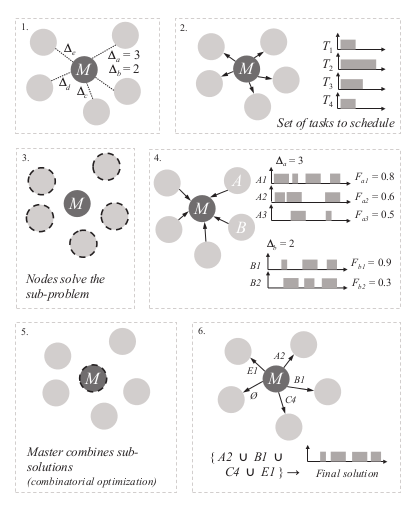
\includegraphics[scale=0.5]{Figures/LGsteps.png} 
\caption{Local-Global policy steps (as extracted from \cite{Araguz15})}
\label{LGsteps}
\end{figure}

To make possible the re-composition of the initial problem and to enable the master to find out the optimal combination taking into account as much information of the \emph{quality} of each local solution as possible, two parameters are defined: the figure of merit \emph{F} and the golden index $ \Delta $. The first of these parameters measures the goodness of each local solution, by combining a number of variables describing it. The second one is the number of possible solutions that each \emph{Local} entity can report to the global layer, and is meant to solve the possibly high heterogeneity in the system: nodes possessing higher processing capabilities will obtain a higher $ \Delta $ than those with lower computational resources.

Having described the basics of the Local-Global algorithm we will now specify the procedure it follows in six steps (see also Fig. \ref{LGsteps}):

\begin{enumerate}
\item \textbf{Characterization.} The $ \Delta $ value for each satellite is assigned, after considering its computing capabilities.
\item \textbf{Task delivery.} Master node selects the time window (duration of the schedule to be produced by the scheduloing algorithm) and discard tasks not fitting within it. After this, it sends to every \emph{Local} entity the set of tasks, so that they can begin to compute sub-solutions.
\item \textbf{Local evaluation.} Local entities' task planners produce as many solutions as its $ \Delta_i $ value, attaching each sub-solution an \emph{F} value.
\item \textbf{Submission of solutions.} Each satellite provides the set of at most $ \Delta_i $ solutions, sending for each one the list of tasks included in that schedule solution and its figure of merit \emph{F}.
\item \textbf{Global selection and combination.} The master triggers a combinatorial optimization process that selects at most one sub-solution per satellite in order to maximize the aggregated \emph{F} value, which is not necessarily the sum of the single \emph{F} values.
\item \textbf{Distribution of solution.} The master answer each \emph{Local} entity with the identity of its selected sub-solution, if any.

In section \ref{LGimplementation} we will focus on the implementation that has been developed in this Bachelor Thesis, specifying the \emph{Local} entity task planner characteristics and the optimization algorithm used in the global layer.
\end{enumerate}
% Chapter Template

\chapter{State of the art} % Main chapter title

\label{Chapter2} % For referencing this chapter elsewhere, use \ref{Chapter2}

%----------------------------------------------------------------------------------------
%	SECTION 1
%----------------------------------------------------------------------------------------

\section{A taxonomy of the existing task scheduler paradigms}

As it was mentioned before, the existing distributed system architectures can be classified according to the grade of centralization, from completely hierarchical systems to fully independent nodes. The research in the distributed algorithms field can also be divided into centralized and non-centralized paradigms, but it cannot be limited to that. However, completely new problems appear in the distributed systems, such as synchronization, leader election or data consistency,  and every different problem opens new approaches and new paradigms.

In particular, into the field of task scheduling, many approaches have been taken. While searching for state-of-the-art algorithms that could be compared with the Local-Global proposal, we found from high-complexity fully-centralized algorithms that may be solved using dynamic or constraint-based programming (meanly for grid-computing or High Performance Computing, as in \cite{anderson2005high,ramamritham1984dynamic,yu2005taxonomy}), to low-computational decentralized schedulers \citep{1310996,zhu2007tasks}.

In the last years, distributed task scheduler research has mainly worked over three different paradigms: \textbf{negotiation or consensus} algorithms, in which nodes in the system \emph{agree} the final schedule --it can be done \emph{offline} as well as \emph{online}--, \textbf{centralized} optimized schedulers --where the degree of centralization can vary-- and more recently \textbf{bio-inspired} approaches --which take profit from observing and imitating the behaviour of the distributed systems present in the nature--.

Of these three categories, the one which almost unexplored is the third one: the research on it is almost only theoretical and only simple and descriptive approaches have been published. Usually they propose a procedure that imitates an observed behaviour on ant colonies or other such distributed \emph{nature} systems. For instance, an adaptation of the stigmergy used by ants to stablish an optimal path is presented in \cite{Stigmergy} and a resources balancing technique extracted from the one observed in ant colonies is described in \cite{antcollonies}. Although these are very interesting approaches, they are still not quite practical for a comparison like the one we want to do.

Completing the classification, our Local-Global policy could be described as a centralized distributed algorithm, while consensus-based distributed task schedulers would be a research-mature third option, fitting our needs for the comparison. As these are actually candidates for the comparison, we will briefly describe in the next section some of the most interesting approaches that have been found, and what are the reasons for having chosen a particular one.

%----------------------------------------------------------------------------------------
%	SECTION 2
%----------------------------------------------------------------------------------------

\section{Comparison: algorithms chosen to test the Local-Global}

Having explored the paradigms that are being investigated in the distributed task scheduler field, we must find out a state-of-the-art algorithm that can be compared with the Local-Global proposal: it should be designed for a similar context and resources requirements.

As it has been already stated, the research in the field of distributed task schedulers is still in its first steps, having that the computational capabilities of nodes in typical distributed systems has been traditionally very low to consider a fully-autonomous system-wide distributed task scheduler running on every node.

The criteria used for choosing the state-of-the-art algorithm to compare the Local-Global with was that it should be as representative of distributed algorithms as possible. Papers presenting such kind of distributed task scheduler are only a few, and sometimes the context is too different to compare our algorithm with (nearly infinite bandwidth, multi-processor scheduling...).

In fact, the context in which the Local-Global policy is meant to work is a very special one: it is a highly-constrained environment in terms of resources and communication, a medium processing capacity (as it is aimed to work on a satellite-on-a-phone nano-satellite, which has higher computing capabilities than standard nano-satellites) and possibly fully independent nodes (depending on the final distributed software architecture).

This reduces our search field: algorithms thought to run on practically infinite communication bandwidth grid computing platforms (as the one presented in \cite{servers}) cannot be compared with the Local-Global.

We cannot also use for the comparison algorithms that are in fact designed to be used for distributed Operating Systems or deploying distributed heavy applications, where the timing requirements are highly-constrained but the communication is practically unlimited \citep{anderson2007consensus,pilloni2012decentralized}. There are also other invalid approaches such as that presented in \cite{luo2013distributed} as it does consider resources requirements in a simple way and the problem resolution is fully centralized, with no participation of the system nodes. However, it presents an auction decision model, something which is also present in the final chosen algorithm.

Two very interesting approaches can be found in \cite{choi2009consensus} and in \cite{bonnet2008coordination}. The contexts are very similar to the ABS satellite constellation. In the first proposal, a combination of consensus and auction-based decision making is used to coordinate a fleet of autonomous vehicles with two decentralized algorithms. Nevertheless, the task description is more complex than the one we need for the ABS case. The second paper describes a communication-constrained based task allocator in the same context of that on ABS project: a satellite constellation. However, the local scheduler of each satellite is not described in the paper, which makes very difficult to be able to use it for comparing with the Local-Global.

Finally, an distributed-architecture-agnostic market-based approach was found in \cite{Edalat09}. The description of the tasks is adequate to what we need and its simplicity yet completeness shows a fully decentralized distributed proposal good for our comparison.

Additionally, a ring-architecture task scheduler algorithm has been designed from the leader election algorithm described in \cite[p.~266]{Tanenbaum:2006:DSP:1202502}. The reason of designing this algorithm was to use a typical distributed structure such as a ring for combining it with the Local-Global policy (as an optimization) in future research.

%-----------------------------------
%	SUBSECTION 1
%-----------------------------------
\subsection{A market-based approach}
\label{sec_MBdescription}

The proposal of \cite{Edalat09} is an adaptive task allocation scheme, which is presented to be used on wireless sensor networks, which is a similar context to that of our initial problem: a resource-constrained environment. A market-based architecture is proposed, in which each node is modelled as a seller who calculates the price for deploying a specific task and offers it to the consumer (the task sender), adapting the price to the changing resources availability for a better energy balance amongst the nodes composing the system. It is important to observe that it schedules the tasks \emph{on the go}, i.e. it is an \emph{online} task scheduler.

In this section a brief description of the presented algorithm, as described in the article mentioned before, is presented, and in \ref{MBimplementation} the details of the implementation carried out in this Thesis will be detailed.

The basic operation of this price-based task allocator is the one that follows: whenever a task arrives to the system, all the nodes in the system are broadcasted the task information. Each node calculates the price it will offer based on his resources and time constraints. High prices mean less energy remaining in the node and/or later processing of the task. Two methods for determining the winner in each round are introduced, having a centralized scheme and a fully distributed one. Results presented in the paper state that the distributed scheme requires less overhead and is more efficient, simply by delaying the price transmission a period of time proportional to the calculated price. This mechanism is further explained later.

The algorithm can be divided in three phases:

\begin{enumerate}
\item \textbf{Listing Phase. } It is proposed a decomposition of an initial set of tasks into a set of smaller sub-tasks forming a task sequence that respects the time constraints and concurrency requirements of the initial group of tasks. Each subtask is represented by an Earliest Start Time (EST, the first time instant in which it can be executed without interfering with its predecessor tasks) and a Latest Start Time (LST, the last time instant in which the task can be begun for letting the successor tasks to be executed). The tasks are queued on a list ordered by their ESTs and LSTs. This queue keeps the order in which the tasks will be broadcasted to the nodes, ready for the task-assignment phase.
\item \textbf{Price-Based Task Assignment Phase. } As it have been stated before, this phase is executed \emph{online}, so the tasks are scheduled  as they arrive in the system. The core of this phase is the price formulation which moreover allows to increase the privacy of the nodes, as they do not transmit the real value of their remaining resources, but only a derived cost.

The parameters that the proposal includes for the price formulation are: task size, energy price, base task price, communication cost, task deadline and processor release time.
\begin{description}
\item[Task Size] ($ S $): the energy needed to process that particular task.
\item[Energy Price] ($ EP $): this value's objective is twofold: to show higher prices for devices with lower energy available (in fact, it is in some way inversely proportional to the instantaneous energy level) and to reflect the cost of recharging the energy. Its value for the node $i$ is defined as:

\begin{equation}
EP_i = \frac{a}{1-e^{E_i/b}}
\end{equation}
 
\item[Base Price] ($ BP $): the computational cost of processing a task in a particular node. It is defined as (node $i$, task $j$):

\begin{equation}
BP_{ij} = S_j \times EP_i
\end{equation}

\item[Communication Cost] ($ CommCost $): the cost of transmitting the output of a task to the node that will process its successor task.

\item[Task Deadline] ($ TD $): the LST already defined in the Listing Phase.

\item[Processor Release Time] ($ RT $): the time at which the task execution would finish if the node finally schedules it.
\end{description}

With all these variables, the proposed price calculation is the one of (\ref{MBPrice1}), with DL the arriving time of the task. This price calculation's goal is to balance the energy consumption among the nodes and to achieve a quicker processing time to more urgent tasks.

\begin{equation}
\label{MBPrice1}
P_{ij} = (CommCost + BP_{ij})\left[1+exp^{\left[\frac{\lambda(t,DL_j)}{\gamma(t,RT_i)}\right]}\right]
\end{equation}


\begin{center}
\begin{tiny}
\begin{minipage}{0.4\textwidth}
$\lambda(t,DL_j) = \left\{ \begin{array}{lrc}
             k(t - DL_j), &   \mathrm{for } & t \geq DL_j \\
             \\ \epsilon &  \mathrm{for } & t \leq DL_j \\
             \end{array}
   \right.$
\end{minipage}\hspace{0.5cm}
\begin{minipage}{0.4\textwidth}
$\gamma(t,RT_i) = \left\{ \begin{array}{lrc}
             k(t - RT_i), &   \mathrm{for } & t \geq RT_i \\
             \\ \epsilon &  \mathrm{for } & t \leq RT_i \\
             \end{array}
   \right. $
\end{minipage}
\end{tiny}
\end{center}

\item \textbf{Recovery Phase. } This phase is intended for recovering from node failures during the task assignment phase, taking into account the existing dependence between tasks.

\item \textbf{Price offering. } Two methods are presented to select the winner bid. Here we will focus on the more efficient decentralized method, as it is the one which we will implement. The core of this procedure is that instead of transmitting to the client the price calculated as soon as it has been obtained, each node waits for a proportional waiting time before broadcasting it to all nodes and goes to a LISTEN mode. If a lower price is received, the node leaves the competition and does not broadcast its bid. Therefore, only the node with lower price effectively sends its bid, reducing the amount of transmitted information.
\end{enumerate}

%-----------------------------------
%	SUBSECTION 2
%-----------------------------------

\subsection{Another ring algorithm}
The leader election algorithm found on \cite{Tanenbaum:2006:DSP:1202502} is a quite simple one, but it is very representative of a typical distributed architecture: the ring structure. We will now describe the design that has been performed in this work to adapt this algorithm for having a distributed task scheduler. Instead of agreeing on who will be the next leader after a leader failure, we want to agree on a schedule for the whole system.

We assume that the satellites in the system are physically (in fact, the ring formation is a practical architecture for satellite constellations) or logically ordered, so that each satellite knows who its successor is, and is able to communicate with it. When a task scheduling process is triggered, the global layer sends to a \emph{master} satellite the set of tasks to be performed. Then the master satellite runs its local scheduler to provide a number of local scheduling sub-solutions for them. Then, it builds up a message with the task set and votes the best sub-solution of those that he has found. The vote consists on \emph{marking} with the sub-solution's \emph{figure of merit} every single task scheduled in that particular sub-solution. This SCHEDULING message is sent to its successor in the ring. At each step, each satellite calculates a number of scheduling sub-solutions and votes the corresponding tasks.

Eventually, the message arrives again to the \emph{master} satellite --he will recognize this message as it will contain its own votes--. Now, the master changes the message type to SOLUTION and looks for the tasks that he had voted. He will effectively assign himself those tasks in which his vote is the highest one. The message goes round the ring again and when it turns to the \emph{master} leader, the scheduling process has finished.

Another variation would be that instead of having only one \emph{voting} round, there would be many of them. At each new round, the satellite would vote the tasks of other calculated sub-solution, if the first task set he voted has been won by other satellite. The algorithm converges to a consensual solution when no more sub-solutions can be voted or every satellite has won the task set it has voted. 
% Chapter Template

\chapter{Design and implementation of a distributed task scheduler} % Main chapter title

\label{Chapter3} % For referencing this chapter elsewhere, use \ref{Chapter3}

%----------------------------------------------------------------------------------------
%	SECTION 1
%----------------------------------------------------------------------------------------

\section{Local-Global implementation}
\label{LGimplementation}

Carrying out a real executable implementation from a more or less theoretical description of an algorithm involves taking some design decisions and choosing programming techniques to achieve an efficient and fair result. A quicker and simpler approach may cause extremely bad results in performance terms. The comparison carried out in this work requires to carefully design the code of both algorithms in order to have an impartial and trustful result.

As a result of this design and implementation process, the first real implementation of this distributed task scheduler has been achieved, being sufficiently complete to derive conclusions on its performance.

In the case of the Local-Global implementation, two clearly different modules have to distinguished: the \emph{Local} entity and the \emph{Global} one. Each one can be described as a unique problem and therefore, each one has to be studied individually.

%-----------------------------------
%	SUBSECTION 1
%-----------------------------------
\subsection{Local algorithm: Adapting a Prolog satellite local scheduler}

%La parte local es un scheduler completamente "local".
%Del ³Cat-1 ya había desarrollado un scheduler local.
%Adaptaciones que se han tenido que hacer: obtener n soluciones, posibilitar que no tenga que incluir todas las tareas, añadir el cálculo de la F (detallar) y comunicación con el global (formato del fichero de output y las entradas).

%If we go back to the description of the Local-Global policy of the section \ref{sec_previouswork}, we can observe that the problem to be solved by each \emph{Local} entity in the Local-Global policy is fully system-agnostic and can be expressed as it follows: given a set \emph{A} of tasks where task $a_j$ has a processing time equal to $l^{a_{j}}$, arrives to the system at $t_0^{a_j}$ and has to be finished before the deadline $t_{\text{max}}^{a_j}$, and a set of resources $R_i$ which will constrain the set of possible schedule solutions, obtain a sub-solution set $P_{i}$ formed by at most $\Delta_i$ schedules that locally meet all the constraints.

The complete independence of this problem from the rest of the system makes it a traditional local task scheduler problem, with the particularity of having to obtain more than one schedule solution for the same set of tasks. This is very important, since it means that most previously designed and implemented local task schedulers applicable to the satellite context can be adapted to satisfy the needs of the \emph{Local} entity in the Local-Global policy. To prove that, different alternatives have been explored. First, an ILOG CPLEX based task scheduler was considered, taking advantage of its performance at solving constrained programming problems. However, a simpler alternative was found: to implement the necessary pieces of code for adjusting an existing local task scheduler used in a previous project of the UPC, the $^3$Cat-1. This local scheduler perfectly fit with the context of the Local-Global policy, as it was specifically designed for a real nano-satellite mission.

This local scheduler of the $^3$Cat-1 project was written in Prolog\footnote{Prolog comes from the french words \textit{PROgrammation en LOGique}, and is a declarative logic programming language}, and is able to solve scheduling problems from a given set of tasks with their time and resource constraints within a scheduling window time $T_w$ and a given set of resources. The main characteristics of this scheduler are:

\begin{enumerate}
\item \textbf{Multi-resource}: the satellite environment defined in this local scheduler has several types of resources that can be required by a task during its execution. In this way, each task requires a certain amount of resource capacity from a certain set of resources. As not all the resources have the same characteristics, the algorithm has to treat them differently. Some examples of the resources that can be defined are: instantaneous power available, accumulated energy, on-board storage, sub-system availability... A classification between \emph{instantaneous} resources and \emph{cumulative} resources is also defined: the completion of a task returns the capacity of an \emph{instantaneous} resource to its initial value, while this is not necessarily true for \emph{cumulative} resources. Examples of \emph{instantaneous} resources are power and sub-system availability. On the other hand, energy and storage are \emph{cumulative} resources.

\item \textbf{Fully elasticity}: the algorithm takes account of the possible variation of the resource capacity, apart from considering the resource consumption required by the tasks. This imposes the use of more constraints, which increases the complexity if the problem to be solved.

\item \textbf{Task priority}: The algorithm handle task priorities to allow the solver to remove low-priority tasks when high-priority ones can be allocated and both do not fit in the same schedule. To do this, an iterative approach is implemented: it generates a valid combination of tasks by gradually expanding an initial sub-problem with more tasks. The addition of new tasks is performed in priority order and starts with the simplest sub-problem: allocate resources to the highest-priority task. After solving this problem, the next task in priority order is added to the list and this new sub-problem is solved. The process is repeated until the iterator reaches the problem containing all the tasks or one of the sub-problems is unfeasible. An example with four tasks, \textbf{a}, \textbf{b}, \textbf{c} and \textbf{d}, sorted in priority order, is shown in Fig. \ref{fig_heuristics}.

\begin{figure}[h!]
\centering
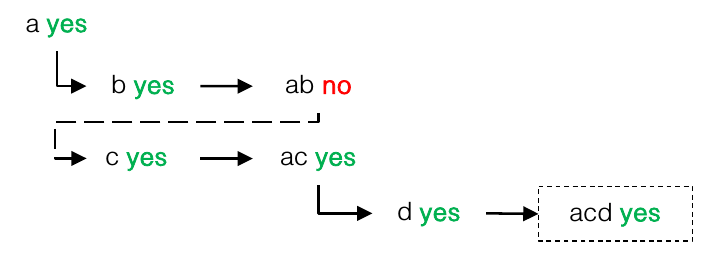
\includegraphics[scale=0.3]{Figures/iterator.png} 
\caption{Example of $^3$Cat-1 local scheduler prioritization heuristics}
\label{fig_heuristics}
\end{figure}

\item \textbf{Task definition}: Task objects contain all the relevant parameters and information for the scheduler. Each task is described with a task identifier, the task priority, and the restrictions for temperature, radiation or position domains. Finally, apart from providing the periodicity and the initial delay, the duration of a task is also defined.  Periodic tasks that should only be scheduled a given number of times, can provide the number of iterations.

\end{enumerate}

Some of these characteristics have to be adapted for the Local-Global context and extended functionalities needed to actually have a practical \emph{Local} entity have to be added. These changes are described below:

\begin{enumerate}
\item \textbf{Calculate $\Delta_i$ scheduling solutions.} Simply repeating the execution of the task scheduler $\Delta_i$ times is not sufficient and neither it is time nor memory efficient. Moreover, it will give $\Delta_i$ identical solutions. The solver must be forced to iterate $\Delta_i$ times for exploring the solutions space and collect a number of them.

The main trouble here is to avoid identical solutions, but the solution is in the core of Prolog's logic: as it is a declarative programming language, its execution procedure is based on checking that the input query can be proven as true according to the input facts and rules that constrain and define the problem. Whenever during the execution of the query an inconsistency is found, backtracking is used to a previous state and explores other possible conditions that are able to satisfy that inconsistency. In this case, this built-in backtracking capabilities could be used to find more than one scheduling solution that satisfies all the constrain.

\item \textbf{Enabling solutions with ``unscheduled'' tasks.} %This iteration process generates a valid combination of tasks by gradually expanding an initial sub-problem with more tasks. It starts with the simplest sub-problem (e.g., ``allocate resources to task $a_1$'') and continuous adding subsequent tasks, backtracking in the combinations tree whenever an unfeasible problem is found.
At the moment, task priorities are not considered for the Local-Global policy. Hence the $^3$Cat-1 \emph{iterator} previously described is not needed. However, without this \emph{iterator} the core solver of this Prolog-based local scheduler is not able to provide a scheduling solution whenever a task set is unfeasible in the given time $T_w$.

The solution to this issue was to expand the scheduling time in such a way that an artificial extra period of time is added to the initial scheduling window. This period of time is special because it has \emph{infinite} resources, so any task can be scheduled within this time. Therefore, whenever a task or a number of them that cannot be scheduled because of resource or time constraints is found, the solver will simply provide a solution with these tasks placed in this extra time period.

\item \textbf{Figure of merit ($F$) definition and calculation.} A main part of the Local-Global policy is the figure of merit, which describes the goodness of each sub-solution reported to the \emph{Global} layer. A critical contribution of this thesis has been a proposal for the definition of $F$. This does not mean only to enumerate a set of variables that can describe the solution, but to study these variables and stablish a valid bounded adaptive combination of all of them depending on each parameter's contribution to the schedule. 

The figure of merit is the sole parameter of goodness information about each sub-solution that the \emph{Global} layer will receive. So, it is the unique information it has to obtain the optimal combination of sub-solutions. Instead of having an extensive knowledge of the resources available in each satellite, it only possesses the figure of merit's value. Because of that, the definition must be as complete as possible, containing all and only the variables that really characterize the sub-solution against any other one. $F$ is completely defined in section \ref{sec_F_LG}.

\item \textbf{Communication with the \emph{Global}.} The local scheduler has been designed to output the first found solution, but the \emph{Local} entity hast to send a set of sub-solutions to the \emph{Global} layer. %As it has been already said, the information that the \emph{Local} must transmit is limited to the subset of tasks included in each sub-solution, and its figure of merit.
For the version implemented in this thesis this communication with the \emph{Global} has been modelled as outputting to a file the $\Delta_i$ solutions found. This files generated by all the \emph{Local} schedulers will be later processed by the \emph{Global} process.

\end{enumerate}

Apart from these added abilities, the $^3$Cat-1 local scheduler was entirely revised and individually tested for ensuring the best performance.

\subsubsection{Formal Local-Global problem description}
\label{sec_F_LG}

The definition of the figure of merit $F$ is essential in the Local-Global policy, as it provides the \emph{goodness} of the global solution.

Let all the terms in the multiple-satellite multiple-task scheduling problem be defined:

\begin{description}
\item[$S$] Number of satellites in the constellation.
\item[$\Delta_i$] Golden number: number of sub-solutions requested to/delivered by satellite $i$. This value is either set dynamically by the global algorithm or generated statically to equalize the computational load in each local scheduler.
\item[$P_{ij}$] The set of sub-solutions generated by satellite $i$ to a given scheduling problem. This term is defined with the pair $\left\langle A_{ij}, F_{ij}\right\rangle$, where
\begin{description}
\item[$A_{ij}$] is the task subset\footnote{Letter $A$ is chosen to prevent confusing the term with time-related variables, denoted with $T$.} included in sub-solution $j$ of satellite $i$ and
\item[$F_{ij}$] is the figure of merit for sub-solution $j$ from satellite $i$.
\end{description}
\item[$T_\mathrm{begin}$] Absolute time at which the scheduling window begins. 
\item[$T_\mathrm{end}$] Absolute time at which the scheduling window ends.
\item[$T_w$] Scheduling time window shared across all satellites, defined as:
\begin{equation}
T_w = T_\text{end} - T_\text{begin}
\end{equation}
\end{description}

Five variables finally form the definition of the figure of merit $F$ value: deadline-based priority, resource utilization, eagerness, satellite processing utilization and responsiveness. This parameters are described below.

Since the Local-Global policy is aimed at planning tasks within the scheduling window $T_w$, the algorithm may yield a final combination of sub-solutions which excludes some tasks. This may be caused either due to their execution domains not being within the current $T_w$ (e.g., a point in the orbit which is never reached by any of the satellites in the constellation) or because the tasks are only present in sub-solutions that are not part of the final global one. In order to deal with this behaviour and to include a prioritization method for tasks with shorter deadlines, the global scheduler will consider a fixed number of future scheduling windows and will promote those solutions where there is a task with sorter deadline\footnote{Deadlines are time values set by ground operators corresponding to the task's $t_{\text{max}}^{a_j}$ value} than that. In order to formulate this feature, let the following terms be defined:
\begin{description}%[leftmargin=1.5cm,labelindent=!]
\item[$L_{ij}$] The minimum distance (in time) between a task deadline and $T_\text{begin}$, for sub-solution $j$ in satellite $i$. 
\item[$N_s$] Number of periods in deadline prioritization. $N_s$ is a static parameter (see (\ref{eq_local-global_deadline_def})). 
\end{description}

Therefore, the \textbf{prioritization term} $\mathbf{D_{ij}}$ can be defined as follows:
\begin{equation}
\label{eq_local-global_deadline_def}
D_{ij} = 
\begin{cases}
2-\dfrac{L_{ij}}{N_s \cdot T_w} & \text{if} \quad L_{ij} \leq N_s \cdot T_w\\
1 & \text{otherwise}
\end{cases}
\end{equation}

Despite the \emph{Global} section of the policy not requiring details about the resources and their capacity allocation to tasks (this is actually what \emph{Local} entities solve), part of a solution's figure of merit ($F_{ij}$), which represents the goodness of a solution, is computed from each satellite's resource usage that derives from each local plan. In order to complete $F$ definition, the capacities and consumptions of each (local) resource are defined:

\begin{description}
\item[$R_i$] Set of resources present in satellite $i$. Therefore, $\bigcup_i{R_i}$ represents the total set of resources of the infrastructure.
\item[$c_{ijk}(t)$] Aggregated\footnote{The sum of resource consumptions by each scheduled task.} consumption of resource $k$ for satellite $i$ and sub-solution $j$ at time $t$.
\item[$m_{ik}(t)$] Capacity of the resource $k$ for satellite $i$ at time $t$.
\end{description}

$\mathbf{C_{ij}}$ is then defined to provide a metric to evaluate sub-solutions in terms of \textbf{resource utilization} as:

\begin{equation}
C_{ij} = \max_{t}\left\lbrace \sum_{k \in R_i}\left(1-\dfrac{c_{ijk}(t)}{m_{ik}(t)}\right)\dfrac{1}{|R_i|}\right\rbrace \qquad C_{ij} \in \left[0,1\right]
\end{equation}

Another variable to evaluate the goodness of a given sub-solution is $\mathbf{G_{ij}}$, which somehow represents the \textbf{eagerness} of the local satellite $i$ with respect to the execution of tasks in sub-solution $j$. A sub-solution will be better if it includes more tasks. However, not all satellites are able to perform every task. Some tasks might have constraints that are impossible to meet for satellites (e.g., a position in the orbit that they never reach) or require the use of specialized instruments which are not common for all satellites. Therefore, the figure of merit needs to evaluate the goodness of a sub-solution with respect to the tasks which each satellite has the capability to execute. In order to do so, $G_{ij}$ is defined as follows:
\begin{description}
\item[$A'_i$] Subset of tasks that satellite $i$ has the capability to perform. If a given satellite is equipped with a resource $k$, but this resource does not have enough capacity to perform a given task, this task will still be present in this subset ($a \in A_i'$).
\end{description}

\begin{equation}
G_{ij} = \dfrac{|A_{ij}|}{|A'_i|}
\end{equation}

Having $G$ and $C$ to evaluate the the number of tasks in a sub-solution and the utilization of resources and $D$ to modify the figure of merit of priority tasks, the following parameters will assess the goodness of a sub-solution with respect to the satellite \textbf{utilization} ($\mathbf{U_{ij}}$) and \textbf{responsiveness} ($\mathbf{E_{ij}}$). 

\begin{eqnarray}
U_{ij} &=& \dfrac{t_{1(ij)}}{T_\text{end}}\\
E_{ij} &=& \dfrac{t_{1(ij)}-t_{0(ij)}}{T_w}
\end{eqnarray}

Where

\begin{description}
\item[$t_0$] Minimum start time among all tasks in sub-solution $j$, corresponding to $\min_{\forall a \in A_i'}{start(a)}$.
\item[$t_1$] Maximum end time among all tasks in sub-solution $j$, corresponding to $\max_{\forall a \in A_i'}{end(a)}$.
\end{description}

These five parameters describe in very different contexts the quality of the sub-solution, providing knowledge of each \emph{Local} entity to the \emph{Global} with small overhead. It should be observed that 	all the parameters are bounded within the interval $\left[0,1\right]$, with the exception of $D_{ij}$, which is bounded within the interval $\left[1,2\right]$. This could be unnecessary as long as every parameter was proportional to the goodness aspect it represents, but is required by the \emph{Global} entity to allow for an efficient optimization. Moreover, this bounding happens to give each parameter a range of values that can vary at most exactly a value equal to $1$, so the relative importance given to each parameter is normalized.

Putting everything together, the \textbf{figure of merit} $\mathbf{F}$ is finally defined as:
\begin{equation}
\label{eq_F_weighted}
F_{ij} = w_c\cdot C_{ij} + w_g\cdot G_{ij} + w_u\cdot U_{ij} + w_e\cdot E_{ij} + w_d\cdot D_{ij} 
\end{equation}

The combination of the five parameters is a weighted sum of their values, Where $w$ are the static weights for each parameter, which can modify the by-default balanced relative importance of each parameter.

%-----------------------------------
%	SUBSECTION 2
%-----------------------------------

\subsection{The Global algorithm}
\label{sec_LG_optimizations}
%Como ya se ha comentado, la capa global es un problema NP-hard de optimización. Complejidad en función de las variables que entran en juego (de forma simple).
%Desarrollo de un algoritmo eficiente: funcionamiento (ordered_list, cuándo cortamos la búsqueda...) gráficas.
%Coordinación con el local.
%Comparación de los tiempos de ejecución para un set aleatorio de sub-soluciones con un algoritmo de fuerza bruta ¡No! Eso va en resultados.

The global scheduling algorithm is basically a combinatorial optimization problem, that can be described as in (\ref{eq_local-global_global_optimization}). The \emph{Global} layer receives sub-solution sets of size $\Delta_i$. Each solution is described by the pair formed by the scheduled tasks set and its figure of merit $\left\langle A_{ij}, F_{ij}\right\rangle$. A potential solution is a combination of at most $S$ sub-solutions, selecting one or none for each satellite. However, it is very important to determine how the combination of sub-solutions can be qualified in terms of the figures of merit of each one of them.

Tthe values could simply be aggregated by summing them, but there is something that must be considered when combining scheduling sub-solutions: a task can appear in more than one sub-solution of the set forming the combination: how does this affect to the quality of this combination as a possible final global solution?

To reflect this degradation in the quality of the global solution, the sum of the $F$ values will be weighted with a multiplying factor that depends on the sum of the number of occurrences of all tasks ($N_b$) normalized to the maximum number of occurrences, which is equal to $S\cdot |A|$, where $S$ is the number of satellites in the constellation and $|A|$ is the number of input tasks. Below the complete definition of the global problem can be found, where the binary decision variables $x_{ij}=1$ if sub-solution $P_{ij}$ is part of the final combination and $0$ otherwise: 

\begin{subequations}
\label{eq_local-global_global_optimization}
\begin{align}
\text{Maximize} \qquad r(P) &= \left(\sum_{i=0}^{S-1}\sum_{j=0}^{\Delta_i-1}x_{ij}{\prod_{f \in F_{ij}}f}\right)\cdot\left(1-\dfrac{N_b}{S\cdot |A|}\right)\\
\text{where:} \qquad N_b &= \sum_{i=0}^{S-1}\sum_{j=0}^{\Delta_i-1}\sum_{k \in A}{B_{ijk}\cdot x_{ij}}\\
B_{ijk} &= \begin{cases}1 & \text{if} ~k \in A_{ij}\\ 0 & \text{otherwise}\end{cases}
\end{align}
\end{subequations}

The description of the \emph{Global} entity implementation is divided in three different subsections: the first one is devoted to briefly analyse the computational complexity of the optimization combinatorial problem to be solved, the second is basically an enumeration of the efficiency-oriented design and recursive improvements made on the algorithm, and finally in the third part the coordination with the \emph{Local} entity is explored. 

\subsubsection{Complexity analysis: an exploding combinatorial problem}

The optimization problem described in (\ref{eq_local-global_global_optimization}) is basically an optimal search problem characterised by mainly three variables: number of satellites $S$, number of sub-solutions provided by each satellite $\Delta$ and the number of scheduling input tasks $|A|$. The entire space of possible combinations is formed by combinations of $S$ elements in which each element is the sub-solution identity selected on each satellite. For instance, for a satellite constellation formed by 5 satellites and having that the first satellite provides 4 sub-solutions, the second provides 3, the third only 2, and both the fourth and the fifth provide 5 sub-solutions, a possible \emph{Global} combination can be represented as (see also Fig. \ref{fig_comb_repr}):

\begin{center}
$ \left(2 0 1 0 3\right) $
\end{center}

This would mean that this particular combination has selected the second sub-solution provided by the first satellite, the first sub-solution provided by the third and the third one from the fifth satellite. Note that it has not selected any sub-solution for the satellites 2 and 4.

\begin{figure}[h!]
\centering
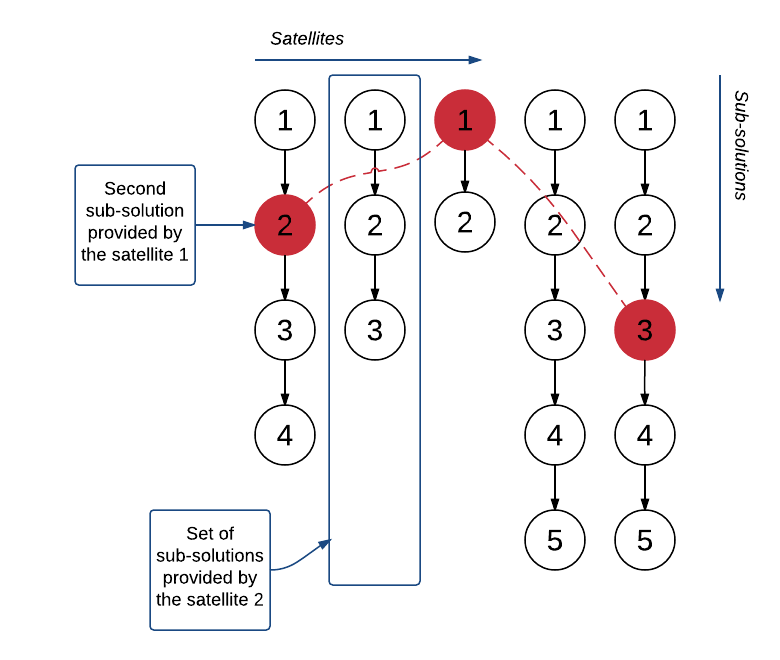
\includegraphics[scale=0.5]{Figures/comb_repr.png} 
\caption{A graphical representation of the combination of several sub-solutions}
\label{fig_comb_repr}
\end{figure}

Summarizing, it can be easily observed that the entire space of combinations would contain $\prod_{i=1}^{S}{\left(\Delta_i + 1\right)}$ combinations, where, for an homogeneous case where $\Delta_i = \Delta_{\text{system}}$, could be approximated to $\Delta_{\text{system}}^S$.

However, this expression does not completely include the complexity of the search. To find out the optimal combination the value of the $r(P)$ function should be calculated for each sub-solution combination, and this calculation depends basically on both the number of input tasks and the number of satellites of the system. This dependence is linear, as one can easily observe that the calculation is fully dominated by the sum of $F$ values, which varies linearly with $S$ (at most exactly $S$ sums must be done) and by the calculation of $N_b$, which depends linearly with the number of tasks $|A|$ (see (\ref{eq_local-global_global_optimization})).

In a basic computational complexity analysis notation, this would lead to a problem dependence on these three variables as shown below:

\begin{equation}
\label{eq_LG_complexity}
Global(\Delta_{\text{system}},S,|A|) \in \Theta\big((\Delta_{\text{system}})^S \cdot  |A|\big)
\end{equation}

\indent To conclude, it can be observed the evolution of the computational complexity when varying only one input with the others kept as a constant value:

\begin{itemize}
\item[--] If both $S$ and $|A|$ are kept constant a \textbf{potential variation} is observed.
\begin{equation}
Global(\Delta,S=S_0,|A|=|A|_0) \in \Theta\big(|A|_0(\Delta_{\text{system}})^{S_0}\big)=\Theta\big((\Delta_{\text{system}})^{S_0}\big)
\end{equation}

\item[--] If $\Delta_{\text{system}}=\Delta_0$ and $|A|$ is kept constant an \textbf{exponential variation} is observed.
\begin{equation}
Global(\Delta_{\text{system}}=\Delta_0,S,|A|=|A|_0) \in \Theta\big(|A|_0(\Delta_0)^S\big)=\Theta\big((\Delta_0)^S\big)
\end{equation}

\item[--] If $\Delta_{\text{system}}=\Delta_0$ and $S$ is kept constant a \textbf{linear variation} is observed.
\begin{equation}
Global(\Delta_{\text{system}}=\Delta_0,S=S_0,|A|) \in \Theta\big(|A|(\Delta_{\text{system}})^{S_0}\big)=\Theta(|A|)
\end{equation}

\end{itemize}

Therefore, an exponentially exploding problem is found when solving the \emph{Global} entity combinatorial optimization.

\subsubsection{An efficiency-oriented design of the combinatorial search}

The most basic and simple solution to this problem would be a brute force approach: exploring the entire space of possible combinations and simply comparing the values of the $r(P)$ function for each of them to finally select the one which maximizes it. However, when facing a problem that depends exponentially as the number of satellites and the $\Delta$ value for each one are increased, the brute force approach can be completely unfeasible.

That is why some efficient improvements have been applied and a careful study on the algorithmics and data structures that could be used has been performed.

To begin with, it is very important to observe two characteristics of the function to be optimized, $r(P)$ (see (\ref{eq_local-global_global_optimization})):
\begin{itemize}
\item It is a bounded function, concretely in the interval $\left[0, W\right]$, where $W$ is the sum of the $F$ weights (see (\ref{eq_F_weighted})): $w_c + w_g + w_u + w_e + w_d\cdot 2$ (remember that $D_{ij}$ is bounded in $\left[1, 2\right]$ instead of $\left[0, 1\right]$).
\item It is formed by the multiplication of two different terms: the sum of $F$ and a weighting value depending on the tasks occurrences, which is also bounded in $\left[0, 1\right]$
\end{itemize}

This means that $r(P)$ itself is bounded in the interval $\left[0, W\right]$ and, what is even more specific, in the interval $\left[1, \mathbb{F}\right]$, where $\mathbb{F}$ is the sum of $F$ of a particular combination.

Therefore, \textbf{finding out the way of exploring the space of combinations in a way that $\mathbb{F}$ value is decreasing, will allow to cut the exploration} as soon as a combination such that its $r(P)$ value is equal to its $\mathbb{F}$ value\footnote{This combination will be proved later to be the optimal combination.}, or a combination which $\mathbb{F}$ value is equal or below the maximum $r(P)$ found till now, is found.

A brief justification of these two affirmations is the one that follows: the fact that $r(P)$ value is bounded in the interval $\left[1, \mathbb{F}\right]$, and that the combinations space is being explored in decreasing $\mathbb{F}$ makes that no combination with lower $\mathbb{F}$ than any other with $r(P) = \mathbb{F}$ will have an $r(P)$ higher than this one because $r(P)$ is never greater than $\mathbb{F}$ (first cutting context) and that no combination with lower $\mathbb{F}$ than the maximum $r(P)$ value found till now will have a higher $r(P)$ than this maximum, for the same reason (second cutting context). In Fig. \ref{fig_r_vs_F} an example of this early searching cut can be seen.

\begin{figure}[h!]
\centering
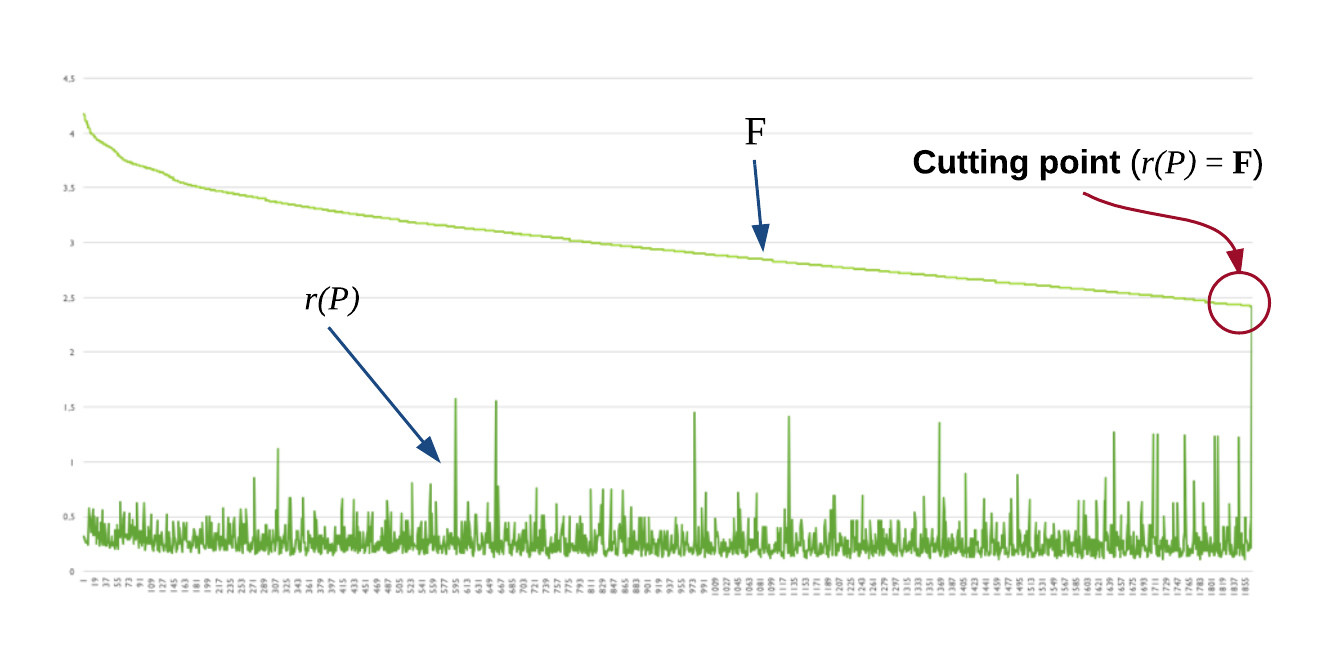
\includegraphics[width=\linewidth]{Figures/r_vs_F.png} 
\caption{Efficient optimal combination search}
\label{fig_r_vs_F}
\end{figure}

The search heuristics designed and implemented to enable a way of exploring the combinations space in decreasing $\mathbb{F}$ is completely explained in Appendix \ref{AppendixB}. In this project, this optimized design has been programmed using C language, and an efficient ordered list library has been also developed in order to have everything in the code controlled for best performance. In chapter \ref{Chapter4}, Fig. \ref{fig_global_brute}, particular results for this implementation compared with a brute force search are shown.

\subsubsection{Coordination with the \emph{Local} entities}

Concluding this section, this part will be devoted to explain the implementation of the \emph{Global}'s process which is in charge of collecting all the solutions submitted by all the \emph{Local} entities and process them for preparing the optimization search described before.

In the simulations performed in this work, the \emph{Local} entities write out in a text file the $\Delta_i$ sub-solutions, detailing for each one the subset of tasks included and the $F$ value.

Therefore, the \emph{Global} has to read that output text files and process them to initialize the internal variables that will represent the satellites' sub-solutions for combining them. If any of the satellites has not been able to send its sub-solutions (e.g., it is down or is not able to communicate with the \emph{Global} entity), the process simply considers it as it had a $\Delta_i = 0$.

At last, this input processing instance orders by descending $F$ value each set of sub-solutions, as the optimized combinatorial search requires.

%----------------------------------------------------------------------------------------
%	SECTION 2
%----------------------------------------------------------------------------------------

\section{Price-based algorithm implementation}
\label{sec_MBimplementation}

In order to implement the algorithm described in \cite{Edalat09}, some implementation details which are not included in the paper (e.g., the system architecture, the communication cost, the scheduling time window...) have been designed. Also some other aspects of the algorithm, such as the price calculation or some synchronization problems, have been improved for a best performance in the tests again the Local-Global policy. In this section the main features of this implementation are described, while in Appendix \ref{AppendixA} all the modifications over the original proposal are detailed.

%-----------------------------------
%	SUBSECTION 1
%-----------------------------------
\subsection{A state graph model}
%Describir el sistema según un grafo de estados.
%Implementación en Erlang, comunicación "real" entre nodos, arquitectura líder-esclavos.
%Ventana de tiempo concreta
%Nada de Listing Phase: sistema simple de dependencias
%Variables que mantiene cada nodo: Communication Cost como distancia entre satélites

A good approach for implementing a distributed algorithm like this is to model each node in the system as a state graph. In this way, programming the nodes is limited to programming all the possible states in the node, the state changes whenever it arrives to the system a particular message (or any other particular event occurs) with the functionalities performed in any of these states and the variables maintained by the node.

In this case, all the \emph{sellers} can be in two different states: WAITING and LISTENING. In the first one, the satellite is ready to begin a scheduling process as soon as a TASK message arrives to the system. In the second state, the system is performing a scheduling process and the node is waiting to transmit its task bid or surrender if a lower-price bid is received from other satellite. The flowchart of the implemented algorithm can be seen in Fig. \ref{fig_state_graph}.

\begin{figure}[h!]
\centering
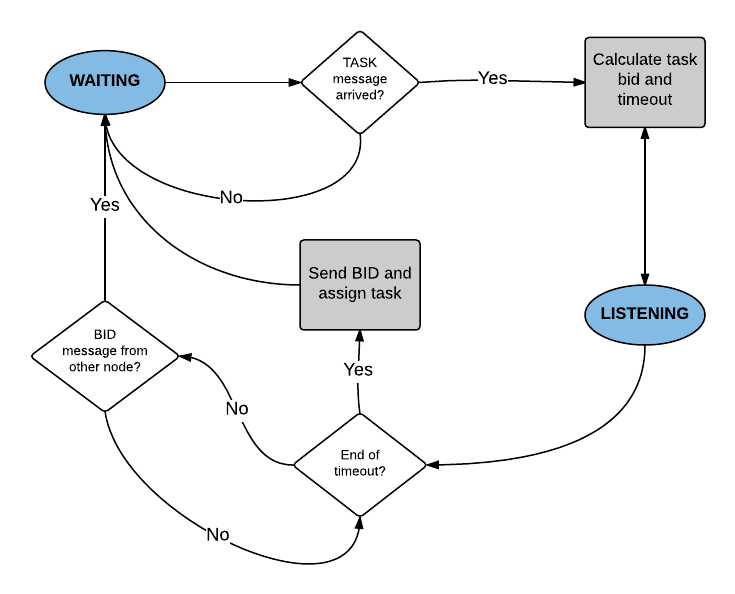
\includegraphics[scale=0.7]{Figures/flow_mb.png} 
\caption{Price-based policy flowchart}
\label{fig_state_graph}
\end{figure}

The auxiliary functionalities that have been implemented are mainly two: the price calculation and the task addition to the local scheduler. The first one is a calculation based on the current state of the node and the second is executed whenever the node has won a scheduling process and assigns itself the task, reserving the corresponding resources and refreshing its own state knowledge.

The node's state knowledge will be now described. In this work the designed set of local variables maintained by each satellite are:

\begin{enumerate}
\item \textbf{Name.} The satellite's ID, used for identifying each satellite's message.
\item \textbf{Energy.} The amount of energy that has not been reserving for executing already assigned tasks.
\item \textbf{Processor release time.} The time instant in which the processor will finish the current scheduled tasks.
\item \textbf{Beginning time.} The initial time of the current scheduling window, used for determining timestamps relative to it, for optimizing the overhead caused by the use of a long absolute time stamp.
\item \textbf{Peers list.} The other satellites' IDs present in the constellation. It also includes the communication cost for each one.
\item \textbf{Schedule.} The local schedule assigned until that particular moment, generated from the different scheduling processes that have been completed since the beginning of the scheduling window.
\item \textbf{Task assignment.} For each already assigned tasks, it contains the ID of the satellite that has been assigned to execute it.
\end{enumerate}

The current implementation has been developed in Erlang code, a functional programming and distributed systems-oriented language. Its distributed nature has allowed to directly simulate different nodes and a real message passing system between the nodes. This truly distributed environment has required a specific architecture design for a better system management.

Because of that, a \emph{leader-slaves} centralized architecture has been implemented. The \emph{leader-slave} relationship is only valid for system registering or de-registering\footnote{Whenever a satellite wants to enter in the system, it has to communicate it to the current leader, and the same for whenever a satellite leaves the system.}, although it is meaningless for the scheduling algorithm.

Another feature of this implementation has been the simplification of the \emph{Listing Phase} (see section \ref{sec_MBdescription}). Instead of dividing complex tasks into simpler ones, an already dependence-processed input task sets has been considered. The dependence among two tasks has been modelled as an added task attribute which contains the ID of its \emph{predecessor} task i.e. the task that must be completed to begin this one. In the next section the task dependence's importance on calculating the task bid on a scheduling process is explained along with other implemented modifications in order to optimize the algorithm.
% Chapter Template

\chapter{Results} % Main chapter title

\label{Chapter4} % Change X to a consecutive number; for referencing this chapter elsewhere, use \ref{ChapterX}

%----------------------------------------------------------------------------------------
%	SECTION 1
%----------------------------------------------------------------------------------------

\section{Parametrizing a distributed task scheduler}
%Para testear hay que tener claro qué variables "barrer"
%Cosas que afectan a la complejidad (tiempo, memoria) del problema: Número de tareas, energía de los satélites, número de satélites, ventana de scheduling,.
%Cosas que afectan al M-B: energía de los satélites y número de tareas: desventaja de un scheduling "secuencializado".
%Cosas que afectan al L-G: Delta! Número de satélites.

In the last section all the details of both Local-Global and price-based distributed task schedulers implementations carried out in this thesis have been detailed. The present section shows the experimental results of the benchmark of simulations that has been performed.

In order to better understand the numeric data, input variables and how these do affect to the time and memory spent in resolving this particular problem must be analysed.

First of all, we will highlight the parameters that affect the general scheduling problem, independent of the particular algorithm chosen to solve it (whether it is the Local-Global or the price-based or any other one):

\begin{itemize}
\item \textbf{Number of tasks.} As the number of tasks to be scheduled increase, the complexity of the problem increases, as with the same available resources (energy, time...) more tasks are to be done. In this sense, the problem is harder to solve.

\item \textbf{Satellite resources.} For the same number of tasks, if the resources available at the system are decreased, the same problem when increasing the number of tasks is found.

\item \textbf{Number of satellites.} Even though this implies having more resources available and hence more possible solutions, an increasing number of satellites translates to a larger distributed system, potentially leading to an unmanageable system full of resources but unable to schedule any task.
\end{itemize}

Secondly, the variables that can particularly influence on the performance of the Local-Global policy will be enumerated:

\begin{itemize}
\item \textbf{Golden index.} This variable is particular to this algorithm. For very high values of the golden index, more sub-solution combinations are possible and, therefore, the complexity of the problem is greater (see (\ref{eq_LG_complexity})). This potential dependence is mitigated in part for low values of golden index thanks to the optimizations of the global combinatorial search.

\item \textbf{Number of satellites.} Although this parameter affects the abstract scheduling problem, it's influence on the Local-Global should be highlighted as the number of sub-solutions combinations to be analysed by the \emph{Global} entity depends exponentially of this variable. This influence is also palliated by the global search.

\item \textbf{Scheduling window.} If the scheduling window time is increased, the task allocation complexity could also increase, as there are more timing combinations available to \emph{test} in the schedule problem. However, if it is set to a very low value, it could create an unsolvable problem, as the same tasks are trying to be scheduled in an insufficient time period.
\end{itemize}

Finally, the price-based algorithm is mainly affected by the following variables:

\begin{itemize}
\item \textbf{Satellites resources.} The results of the algorithm can be quite poor in terms of optimality of the final schedule when the satellite have not much resources, because this lead to high bid calculations and therefore to large scheduling process times and less scheduled tasks.

\item \textbf{Number of tasks.} The main drawback of price-based is the sequential nature of the scheduling process: each task is processed and scheduled in non-overlapping rounds, so a high number of tasks could lead to an overloaded system not able to schedule tasks at the same velocity that they arrive in the system.
\end{itemize}

Sweeping these parameters will show the behaviour of each algorithm and its input limits (i.e. the limits on the input's complexity for the algorithm to be able to solve it in a reasonable period of time and spending a reasonable amount of memory). This previous analysis shall be confirmed by the experimental simulations presented in this section.

\section{Performance Tests}

Having theoretically enumerated the critical variables which contribute to the complexity of each algorithm, experimental simulations have been carried out.

A simple tester application has been implemented, in order to have a suitable testing platform to perform extensive simulations and sweeps of the critical variables to capture statistical measures. This application receives the set of input variables (number of satellites, number of tasks, golden index, scheduling window...) and the required sweep. It then simulates an Erlang execution with random generated tasks satisfying the input parameters and, after that, it simulates a Local-Global environment, using the same task set for both. Finally, it measures the time and memory expense and reports it to an output file, in such a format that can be easily processed by a Matlab script. Each simulation is performed several times in order to extract the statistical information: the mean and standard deviation for each of the measured variables.

%% FIGURITA del tester

Six main test sets have been performed: three tests in which one out of the main critical variables (i.e. number of satellites, number of tasks and golden index) have been fixed; and three tests sweeping only one of the three variables in order to find the limits on the problem size for each algorithm to be able to solve it\footnote{The sweeping ranges and the fixed values are chosen from the most representative cases.}:
\begin{enumerate}
\item In the first benchmark, the number of satellites is swept from 1 to 5 and the golden index\footnote{Note that the golden index for the price-based policy is irrelevant.} is swept from 1 to 7, having fixed the number of tasks to 15.

\item In the second benchmark, the number of satellites is swept from 1 to 5 and the number of tasks is swept from 1 to 30, having fixed the golden index to 4.

\item In the third benchmark, the number of satellites is fixed to 5 while the golden index is swept from 1 to 7 and the number of tasks is swept from 1 to 30.

\item The fourth benchmark fixes both number of satellites and golden index to 5 and 4, respectively. The number of tasks is swept from 10 to 100 in steps of 10 tasks.

\item The fifth benchmark sweeps the golden index from 5 to 20 in steps of 5 while fixing the number of satellites to 5 and the number of tasks to 15.

\item The sixth benchmark explores a number of satellites sweep from 1 to 14\footnote{A distributed satellite environment with more than 14 satellites could not be simulated with the computer available for the tests because of memory constraints.} while fixing the number of tasks to 15 and the golden index to 2.
\end{enumerate}

All the tests were performed with a scheduling time window of 90 minutes and the duration of the tasks was randomly chosen as a value from 1 to 2 minutes. The execution time shown in the plots is referred to the time spent in scheduling tasks during the whole scheduling window. All the satellites in the system have the same amount of resources: the needed power to be permanently processing tasks. The 2D plots reflect the error bars and envelope error functions\footnote{These envelope functions are plotted with discontinuous lines.} for the standard deviation calculated from each one of the simulations.

For a better comprehension and analysis of each one of the simulations performed, the results will be shown in three different sections: first the Local-Global policy and the price-based results are separately analysed, and finally both are compared.

%-----------------------------------
%	SUBSECTION 1
%-----------------------------------
\subsection{Local-Global}

The time spent in solving each problem of the benchmark is shown in figures \ref{fig_tLG_satsfix}, \ref{fig_tLG_tasksfix} and \ref{fig_tLG_goldenfix}. It can be observed that for this values of number of satellites and golden index the time is almost constant, thanks to the optimizations that have been implemented in the \emph{Global} entity, explained in section \ref{sec_LG_optimizations}. However, the number of tasks causes a linear growth in the execution time.

A similar analysis can be done in terms of memory usage: the global combinatorial search optimizations reduce the effects of increasing the number of satellites (the memory used when sweeping this variable is nearly constant) and the golden index (in this case, the memory increases linearly with a small slope). The memory consumption for each test can be seen in figures \ref{fig_mLG_satsfix}, \ref{fig_mLG_tasksfix} and \ref{fig_mLG_goldenfix} respectively.

\begin{figure}[h!]
  \begin{minipage}[b]{0.5\linewidth}
    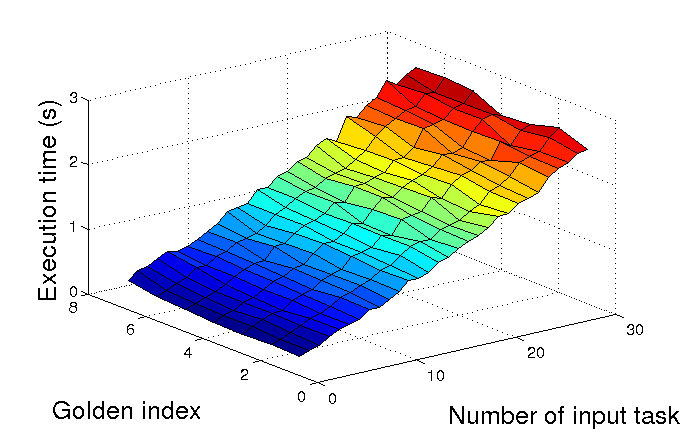
\includegraphics[width=\linewidth]{Figures/tLG_satsfix.png}
    \caption{Local-Global: execution time (satellites fixed)}\label{fig_tLG_satsfix}
  \end{minipage}  
  \begin{minipage}[b]{0.5\linewidth}
    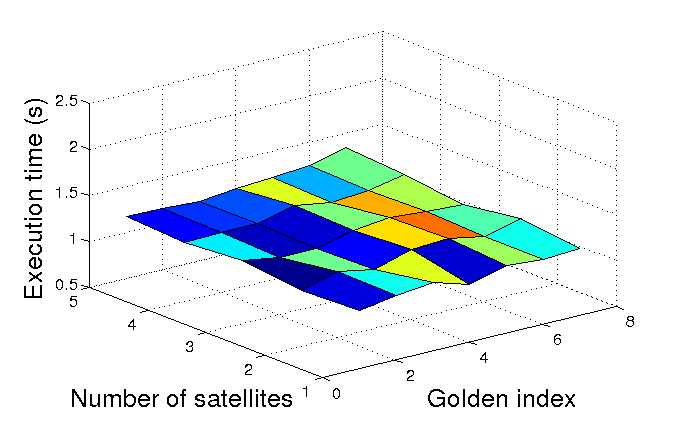
\includegraphics[width=\linewidth]{Figures/tLG_tasksfix.png}
    \caption{Local-Global: execution time (input tasks fixed)}\label{fig_tLG_tasksfix}
  \end{minipage}  
\end{figure}
\begin{figure}[h!]
  \begin{minipage}[b]{0.5\linewidth}
    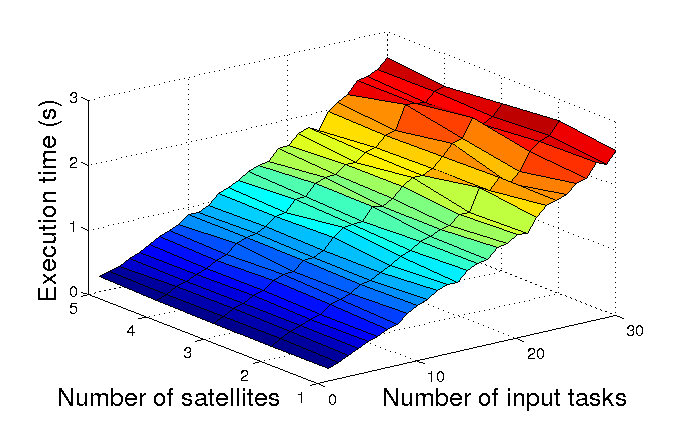
\includegraphics[width=\linewidth]{Figures/tLG_goldenfix.png}
    \caption{Local-Global: execution time (golden index fixed)}\label{fig_tLG_goldenfix}
  \end{minipage}
    \begin{minipage}[b]{0.5\linewidth}
    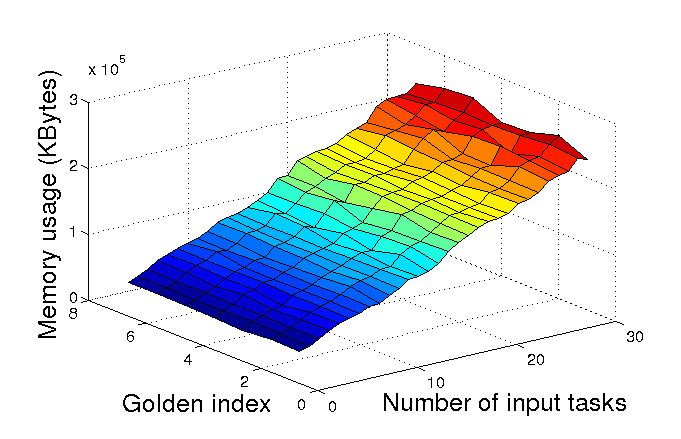
\includegraphics[width=\linewidth]{Figures/mLG_satsfix.png}
    \caption{Local-Global: memory usage (satellites fixed)}\label{fig_mLG_satsfix}
  \end{minipage}
\end{figure}
\begin{figure}[h!]
  \begin{minipage}[b]{0.5\linewidth}
    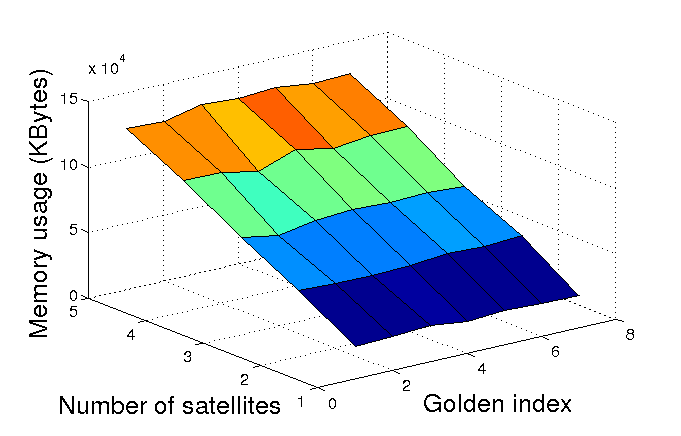
\includegraphics[width=\linewidth]{Figures/mLG_tasksfix.png}
    \caption{Local-Global: memory usage (input tasks fixed)}\label{fig_mLG_tasksfix}
  \end{minipage}  
  \begin{minipage}[b]{0.5\linewidth}
    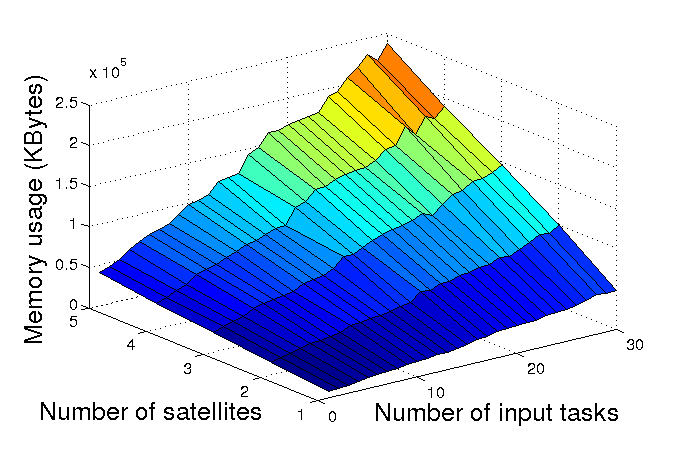
\includegraphics[width=\linewidth]{Figures/mLG_goldenfix.png}
    \caption{Local-Global: memory usage (golden index fixed)}\label{fig_mLG_goldenfix}
  \end{minipage}
  \hfill
\end{figure}

However, the improvement achieved for low values of satellites and golden index for time and memory measures is not preserved for high values, as it can be observed in figures \ref{fig_tmLG_slim}, \ref{fig_tmLG_alim}, and \ref{fig_tmLG_glim}. Nevertheless, the linear dependence from input tasks is kept.

\begin{figure}[h!]
  \begin{minipage}[b]{\linewidth}
    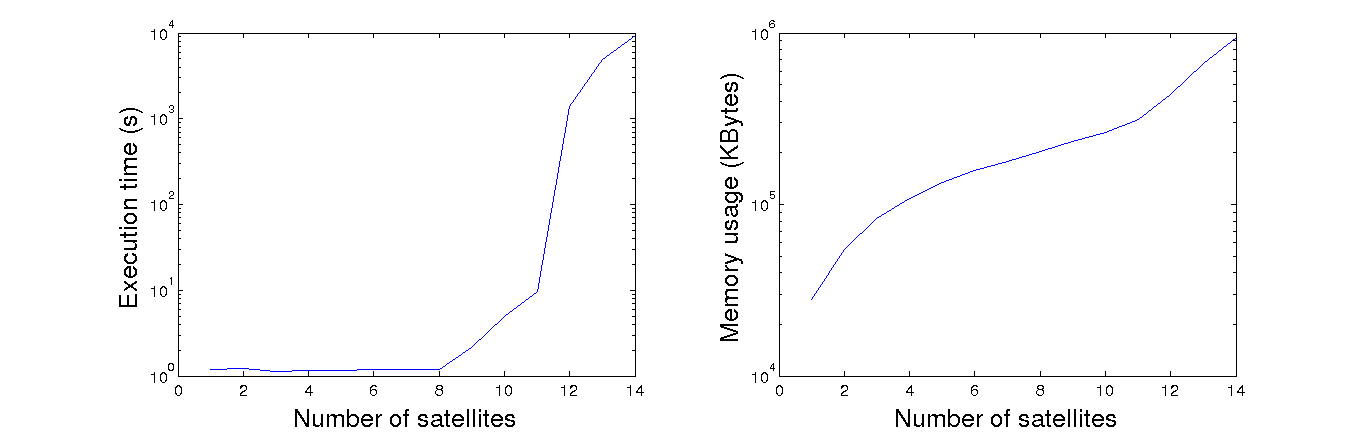
\includegraphics[width=\linewidth]{Figures/tmLG_slim.png}
    \caption{Local-Global: execution time and memory usage (varying number of satellites)}\label{fig_tmLG_slim}
  \end{minipage}
  \end{figure}
\begin{figure}[h!]
  \begin{minipage}[b]{\linewidth}
    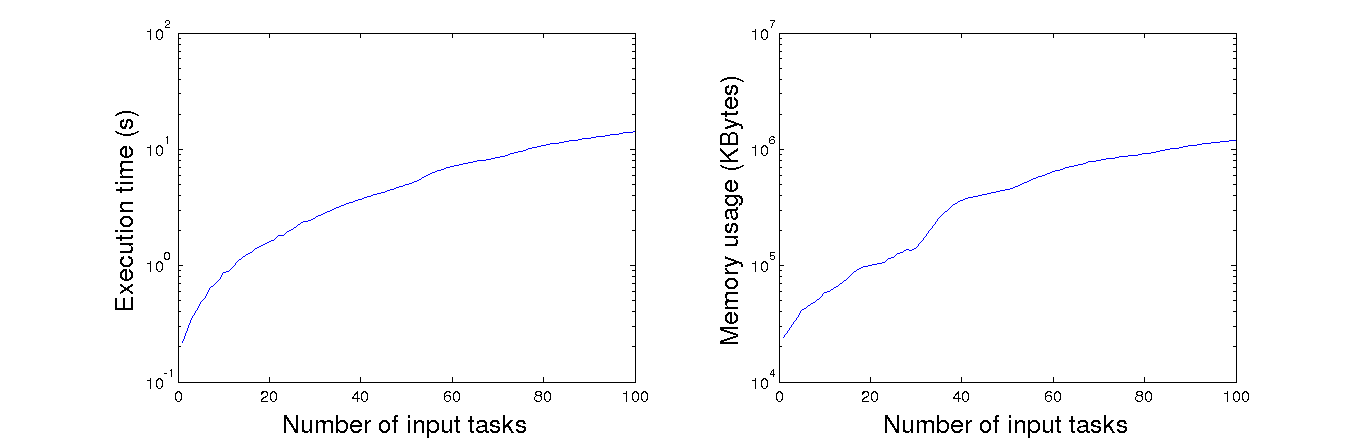
\includegraphics[width=\linewidth]{Figures/tmLG_alim.png}
    \caption{Local-Global: execution time and memory usage (varying number of input tasks)}\label{fig_tmLG_alim}
  \end{minipage}  
\end{figure}
\begin{figure}[h!]
  \begin{minipage}[b]{\linewidth}
    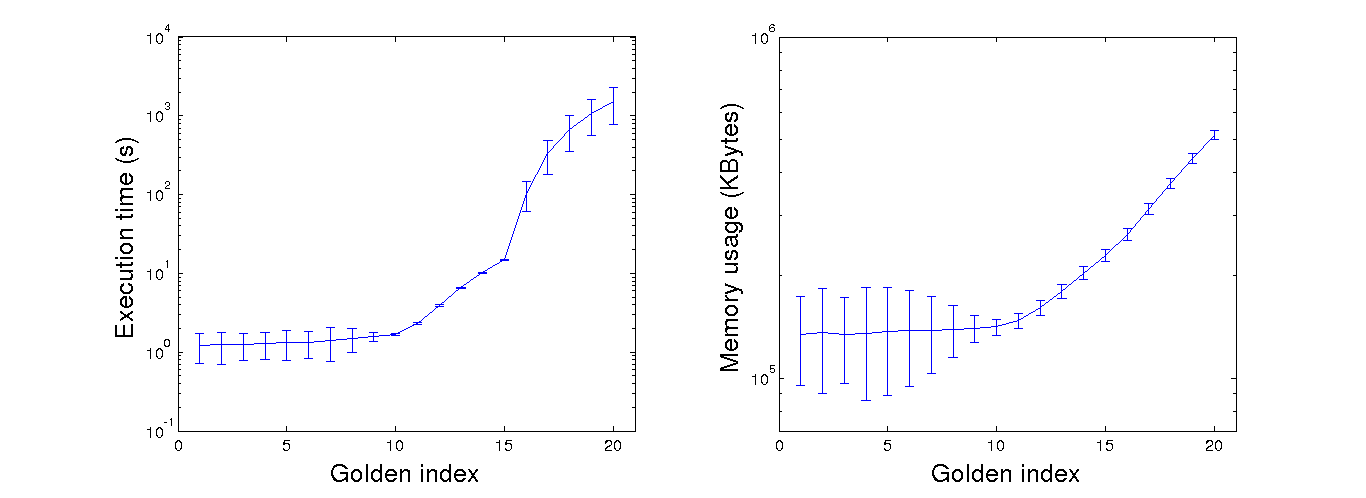
\includegraphics[width=\linewidth]{Figures/tmLG_glim.png}
    \caption{Local-Global: execution time and memory usage (varying golden index)}\label{fig_tmLG_glim}
  \end{minipage}
  \hfill
\end{figure}

Finally, the number of total scheduled tasks (i.e. the number of tasks that are present in the final schedule solution) is represented in figures \ref{fig_aLG_satsfix} (number of satellites fixed) and \ref{fig_aLG_goldenfix} (golden index fixed). Both plots are very similar and highlight an important characteristic of the Local-Global policy with the implementation carried out in this thesis: for less than 10 input tasks (in this particular benchmark) the system achieves a final schedule which schedules all the tasks available. Then, the system begins to saturate and it is not able to schedule all the input tasks. However, the ability of scheduling more tasks at high number of input tasks increases, but not at the same rate than the one of the input tasks. In Fig. \ref{fig_aLG_alim} a final constant saturation point at 80 input tasks can be observed. This behaviour can be optimized by enhancing the \emph{Local} entity so it sends better sub-solutions, as the one implemented for this Thesis still produces some suboptimal sub-solutions that affect the combining capabilities of the \emph{Global}.

\begin{figure}[h!]
  \begin{minipage}[b]{0.5\linewidth}
    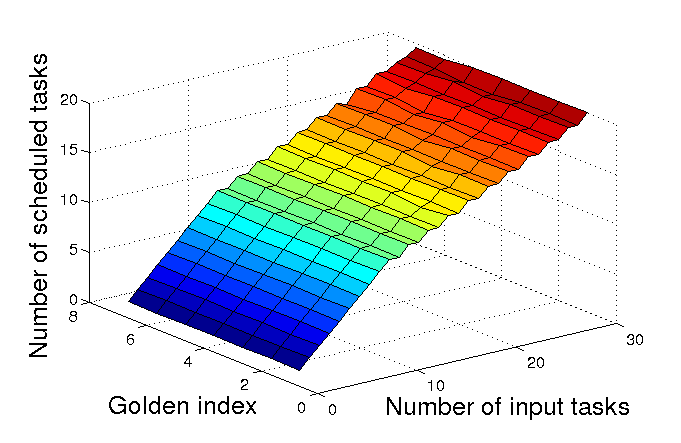
\includegraphics[width=\linewidth]{Figures/aLG_satsfix.png}
    \caption{Local-Global: scheduled tasks (satellites fixed)}\label{fig_aLG_satsfix}
  \end{minipage}   
  \begin{minipage}[b]{0.5\linewidth}
    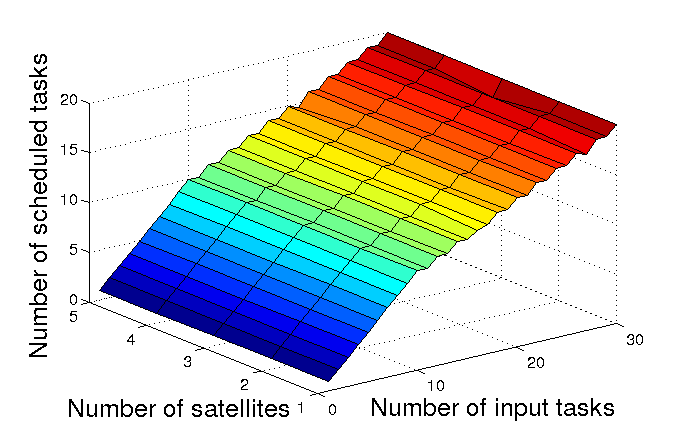
\includegraphics[width=\linewidth]{Figures/aLG_goldenfix.png}
    \caption{Local-Global: scheduled tasks (golden index fixed)}\label{fig_aLG_goldenfix}
  \end{minipage}
\end{figure}
\begin{figure}[h!]
  \begin{minipage}[b]{\linewidth}
  \centering
    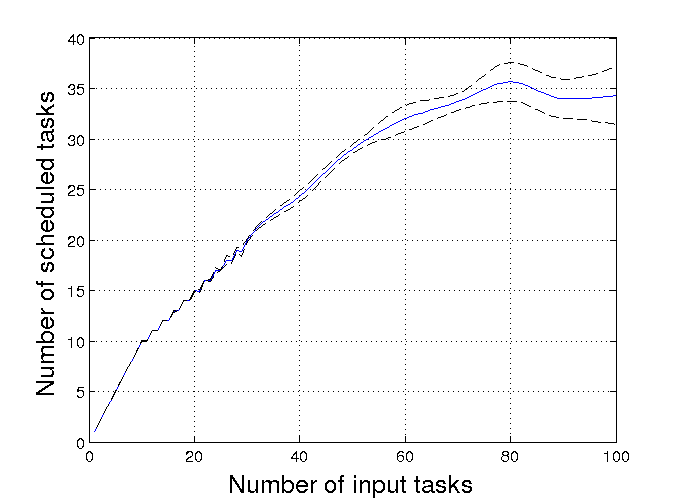
\includegraphics[width=0.6\linewidth]{Figures/aLG_alim.png}
    \caption{Local-Global: scheduled tasks for large input tasks range}\label{fig_aLG_alim}
  \centering
  \end{minipage}
  \hfill
\end{figure}

In this policy, special attention to the global combinatorial search optimizations has to be paid. In order to quickly analyse the improvement that represents to the entire policy, a performance comparison with a brute-force search has been carried out. Results are shown in Fig. \ref{fig_global_brute}, where the mitigation (in the optimized version) of exponential increase with the problem size is clearly observed.

\begin{figure}[h!]
  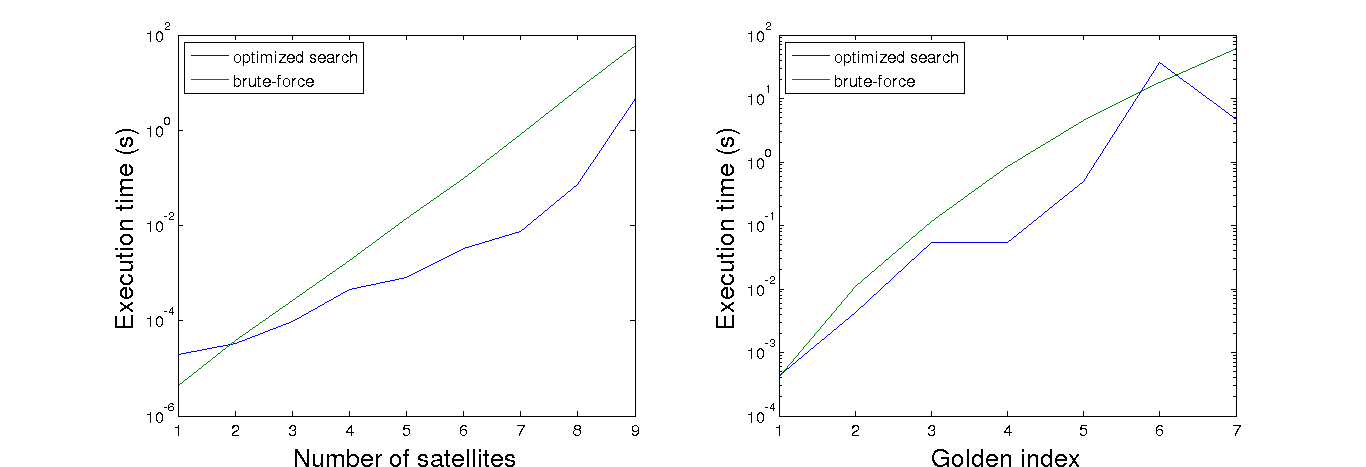
\includegraphics[width=\linewidth]{Figures/global.png}
  \caption{Global optimization: execution time comparison (combinatorial search vs. brute-force)}\label{fig_global_brute}
\end{figure}

%-----------------------------------
%	SUBSECTION 2
%-----------------------------------

\subsection{Price-based}

The price-based results are simpler, as there are only two main variables to sweep: number of satellites and number of tasks. The test results are shown in Fig. \ref{fig_tMB_sw} for time measures, in Fig. \ref{fig_mMB_sw} for memory measures and in Fig. \ref{fig_aMB_sw} for scheduled tasks number.

Regarding time and memory, a clear influence of the increase in the number of tasks is observed, while the number of satellites do not affect the final result. The results in the finally scheduled number of tasks must be highlighted: the price-based algorithm achieves to schedule almost all the input tasks for this values. However, when it is swept over the number of tasks at high values (see Fig. \ref{fig_aMB}), it can be very clearly observed that the performance decreases completely for more than 30 input tasks.

\begin{figure}[h!]
  \begin{minipage}[b]{0.5\linewidth}
    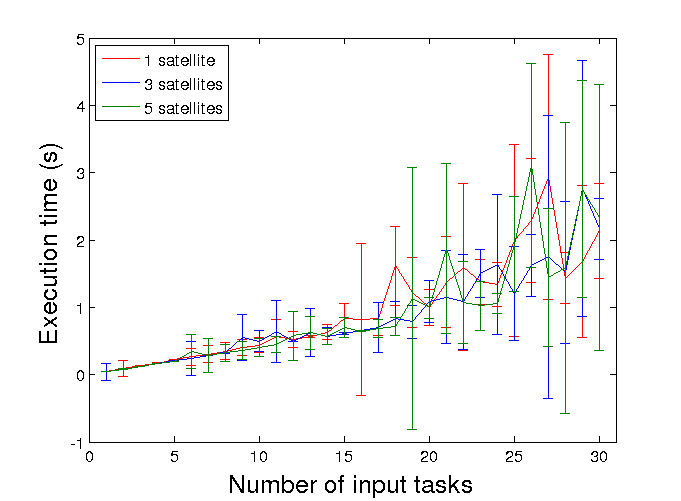
\includegraphics[width=\linewidth]{Figures/tMB_sw_2.png}
    \caption{Price-based: execution time}\label{fig_tMB_sw}
  \end{minipage} 
  \begin{minipage}[b]{0.5\linewidth}
    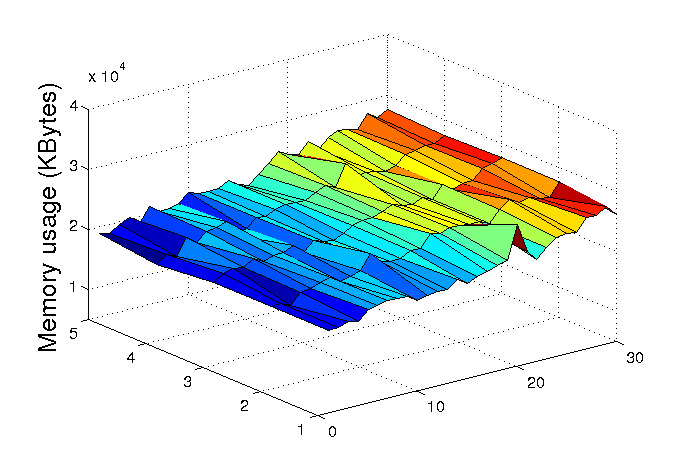
\includegraphics[width=\linewidth]{Figures/mMB_sw.png} 
    \caption{Price-based: memory usage}\label{fig_mMB_sw}
  \end{minipage} 
\end{figure}
\begin{figure}[h!]
  \begin{minipage}[b]{0.5\linewidth}
    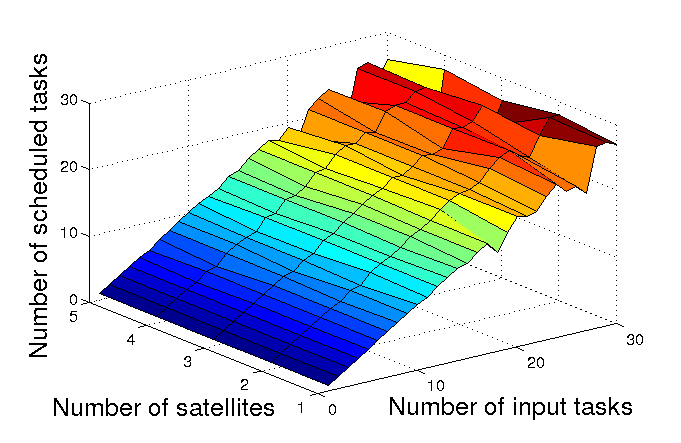
\includegraphics[width=\linewidth]{Figures/aMB_sw.png}
    \caption{Price-based: scheduled tasks}\label{fig_aMB_sw}
  \end{minipage}
    \begin{minipage}[b]{0.5\linewidth}
    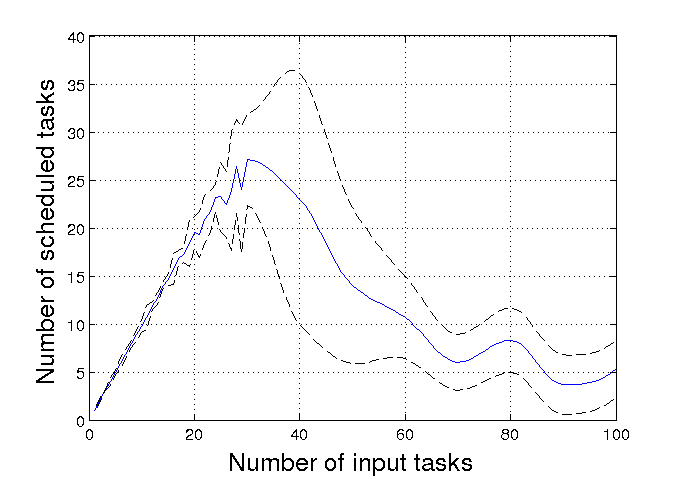
\includegraphics[width=\linewidth]{Figures/aMB.png}
    \caption{Price-based: scheduled tasks for large input tasks range}\label{fig_aMB}
  \end{minipage}
  \hfill
\end{figure}

\clearpage

%-----------------------------------
%	SUBSECTION 3
%-----------------------------------

\subsection{The comparison}

As a first concluding result, some comparison representations are shown below, highlighting now the difference in the behaviour of both schedulers that analysing separately each one can remain out of the sight.

Regarding the time spent in solving the input tests, it can be observed in Fig. \ref{fig_tLGMB} that both increasing the number of satellites or the number of tasks in the system, the price-based scheduler has lower execution times for almost all the cases. Moreover, the Local-Global policy tends to increase exponentially the resources it spends. The memory utilization behaviour is very similar to the time measures (see Fig. \ref{fig_mLGMB}).

However, it can be observed that the Local-Global policy demonstrates its strength by obtaining a constant throughput in terms of scheduled tasks (besides other parameters of the solution quality such as satellite utilization or responsiveness) when increasing the number of input tasks (see Fig. \ref{fig_aLGMB}): it achieves scheduling more tasks than the price-based scheduler for almost all the tests. The range in which the price-based performs better than the Local-Global is from 10 to 40 tasks (i.e. between the first saturation point of the Local-Global and the saturation point of the price-based).

\begin{figure}[ht]
  \begin{minipage}[b]{\linewidth}
    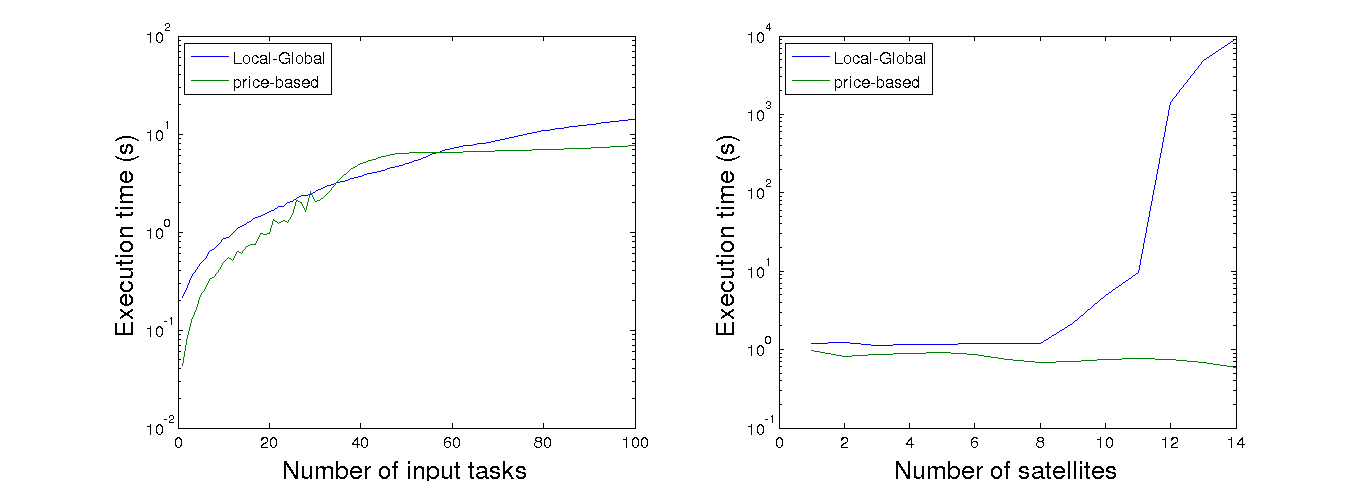
\includegraphics[width=\linewidth]{Figures/tLGMB.png}
    \caption{Local-Global vs price-based: execution time comparison}\label{fig_tLGMB}
  \end{minipage} 
\end{figure}
\begin{figure}[h!]
  \begin{minipage}[b]{\linewidth}
    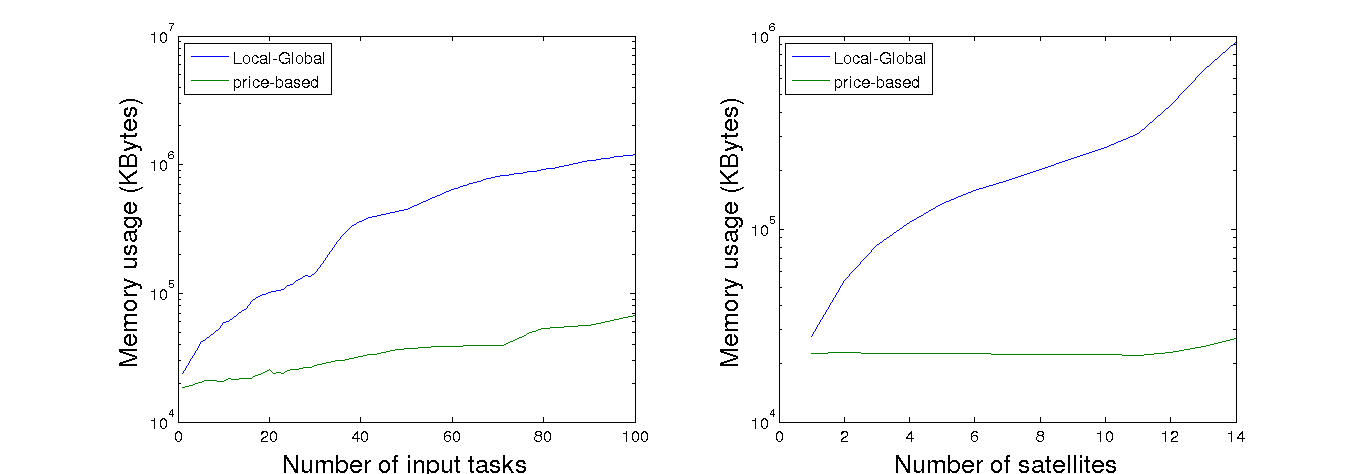
\includegraphics[width=\linewidth]{Figures/mLGMB.png} 
    \caption{Local-Global vs price-based: memory usage comparison}\label{fig_mLGMB}
  \end{minipage} 
\end{figure}
\begin{figure}[ht!]
  \begin{minipage}[t]{\linewidth}
  \centering
    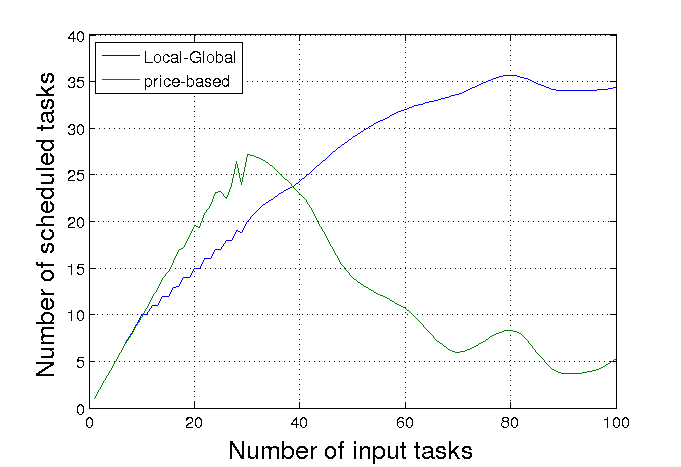
\includegraphics[width=0.6\linewidth]{Figures/aLGMB.png}
    \caption{Local-Global vs price-based: scheduled tasks comparison}\label{fig_aLGMB}
  \centering
  \end{minipage}
  \hfill
\end{figure} 
%% Chapter Template

\chapter{Conclusions} % Main chapter title

\label{Chapter5} % For referencing this chapter elsewhere, use \ref{Chapter5}

%----------------------------------------------------------------------------------------
%	SECTION 1
%----------------------------------------------------------------------------------------

\section{Results analysis and solutions quality}

In the last section the most significant results have been shown. However, some specificities of each algorithm that we may not observe in those figures must have been explained for a better comprehension of the behaviour, advantages and disadvantages of each algorithm.

Regarding the Local-Global policy, it must be said that there are many solutions quality aspects included in the schedule optimization it performs apart from how many tasks have been finally scheduled (remember section \ref{sec_F_LG}). Moreover, the tasks can be scheduled concurrently and any resource definition can be introduced in the problem definition. Finally, the golden index can be optimized for each satellite, either statically or dynamically by the \emph{Global} instance. This can model much better the heterogeneity among the satellites. In fact, homogeneity in the system deteriorates the results of the Local-Global, as very similar sub-solutions are delivered to the \emph{Global} from several satellites, giving no chance to find a good combination.

The price-based scheduler has also some characteristics that are not found on Local-Global: dependence between tasks and accounting the communication cost of passing the results from one task to another is included in the schedule calculation. Furthermore, the market model allows us to redefine the bid calculation for taking into account whichever parameter we want to adapt the performance to a particular system. This could be done also either statically or dynamically.

When both algorithms are compared, we find that the price-based execution times and memory usage is lower than the Local-Global's, but there are some handicaps to be observed: the price-based ``sequentilaization'' of the scheduling process is a bottleneck and causes a saturation point that decreases the performance for high number of input tasks, while the Local-Global's saturation is softer and it achieves to maintain the number of scheduled tasks for this situation. Price-based scheduler also requires good communication among the satellites forming the cluster, something not very realistic in a highly-constrained bandwidth context such as the open space. The Local-Global's poor performance for high values of number of satellites and golden index can be improved by optimizing the \emph{Local} entity and smartly adapting the values of the golden index.

\section{Future work}

In this work the Local-Global policy's design has been completed and fully implemented, finding out and implementing the most appropriate state-of-the-art system for comparing both and test the real Local-Global's performance. The parameters fitting most to the comparison's goals have been defined and large testing benchmarks have been performed for both algorithms, quantitatively measuring the behaviour of each one of them.

These complete work allows us to firmly state some conclusions about the Local-Global policy's future work to be done:
\begin{itemize}
\item As it has already been said, although the current performance can be considered as a very good result for the first approach, an improvement can be obtained by optimizing the \emph{Local} scheduler. The optimization of this scheduler should be done on the sub-solutions generation: although each sub-solution, if considered on its own, is a good result, obtained in very low time, the whole set of $\Delta_i$ sub-solutions are not optimal, as they may not be the best sub-solutions to be found, and the may contain repetitions among them.
\item Also some optimizations could be included in the \emph{Global} combinatorial search. Despite having very good performance when heterogeneous satellites form the cluster, for homogeneous cases it decreases dramatically. These are the cases to be studied for the improvements to be carried in the algorithm.
\item Task dependence defined in the price-based scheduler could be included in the policy, as it is a practical functionality to be implemented for small tasks forming an entire mission or activity.
\end{itemize}

To conclude, the results obtained in this Bachelor Thesis have allowed to characterize a theoretical sketched distributed task scheduler that could be implemented as a critical part of the autonomy system of future fractionated satellite systems. 

%----------------------------------------------------------------------------------------
%	THESIS CONTENT - APPENDICES
%----------------------------------------------------------------------------------------

\appendix % Cue to tell LaTeX that the following "chapters" are Appendices

% Include the appendices of the thesis as separate files from the Appendices folder
% Uncomment the lines as you write the Appendices

% Appendix A

\chapter{Appendix Title Here} % Main appendix title

\label{AppendixA} % For referencing this appendix elsewhere, use \ref{AppendixA}

Write your Appendix content here.
%% Appendix A

\chapter{Search heuristics for the Global algorithm} % Main appendix title

\label{AppendixB} % For referencing this appendix elsewhere, use \ref{AppendixA}

In section \ref{sec_LG_optimizations}, the efficient-oriented implementation of the combinatorial optimization problem that has to be solved by the Global algorithm is described. A way of exploring the space of combinations in decreasing $\mathbb{F}$ is needed to efficiently search for the optimal combination. In this appendix, the designed search heuristics to solve this problem are explained.

First of all, it must be assumed that the $S$ lists of $\Delta_i$ sub-solutions delivered by each satellite are ordered by decreasing $F$. This means that combination $\left(1 1 ... 1)\right)$ is the one which has the highest $\mathbb{F}$ value. However, this does not imply that this combination is the one that has a maximum $r(P)$ value.

Therefore, to explore the combinations space in decreasing $\mathbb{F}$, the combination $\left(1 1 ... 1)\right)$ has to be be the first one. The way to follow the exploration is explained below.

Let two key concepts for this explanation be defined (see also Fig. \ref{fig_succ}):
\begin{itemize}
\item A combination's \textbf{successor} is any other combination that is the selection of exactly the same sub-solutions as the first one except by one and only one satellite, for which it has selected the sub-solution immediately following the one that has selected the first combination in order of decreasing $\mathbb{F}$. For instance, the combination $\left(\mathbf{3} 3 2 4 0)\right)$ is the successor of $\left(2 3 \mathbf{2} 4 0)\right)$. Observe, however, that it is also successor of $\left(3 \mathbf{2} 2 4 0)\right)$.
\item In the same way, a combination's \textbf{predecessor} is any other combination that is the selection of exactly the same sub-solutions as the first one except by one and only one satellite, for which it has selected the sub-solution immediately preceding the one that has selected the first combination in order of decreasing F. $\left(2 3 \mathbf{2} 4 0)\right)$ and $\left(2 \mathbf{2} 2 5 0)\right)$ are predecessors of $\left(2 \mathbf{3} 2 \mathbf{5} 0)\right)$.
\end{itemize}

\begin{figure}[h!]
\centering
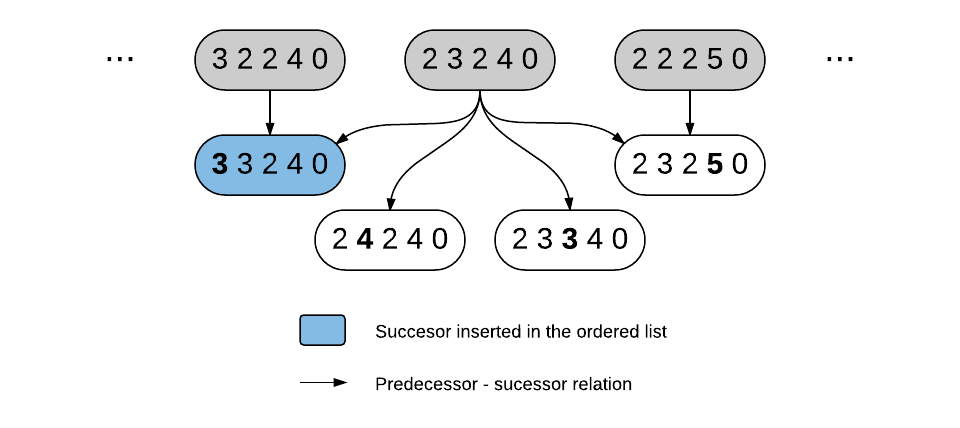
\includegraphics[scale=0.7]{Figures/succ.png} 
\caption{Predecessor and sucesors in the combinations space}
\label{fig_succ}
\end{figure}

Therefore, it can be proven that the exploration of the combinations space will be performed in decreasing $\mathbb{F}$ with the following procedure: for each combination being processed its successors are inserted in an ordered list and the first element in the list is selected as the following combination to be processed, starting from the combination $\left(1 1 ... 1)\right)$.

Noteworthy, a combination has more than one predecessor, so it would be inserted more than once in the ordered list, and hence it would be unnecessarily processed more than once. In order to insert the elements once and only once in the ordered list, each combination selects the successors to be inserted in the following way (see also the example of Fig. \ref{fig_succ}): from all the set of successors of a combination $c$ of the form $\left(1 1 ... c_k ... c_n)\right)$ where $c_k \in [2, \Delta_i]$ and $k \in [1,n]$, the inserted combinations subset is formed by all the successors of $c$ which differ from $c$ in any of the first $k$ components / satellite sub-solutions selections (e.g., the combination $(1 1 4 2 6)$ would insert $(2 1 4 2 6)$, $(1 2 4 2 6)$ and $(1 1 5 2 6)$).
%\input{Appendices/AppendixC}

%----------------------------------------------------------------------------------------
%	BIBLIOGRAPHY
%----------------------------------------------------------------------------------------

\printbibliography[heading=bibintoc]

%----------------------------------------------------------------------------------------

\end{document}  
